\documentclass[aspectratio=169]{beamer} % [mathserif]
\usepackage{amsmath}
\usepackage{graphicx}
\usepackage{subfigure}
\usepackage{wrapfig}
\usepackage{booktabs}
\usepackage{hyperref}
\usepackage{media9}
% \usepackage{pgfplots}
% \pgfplotsset{compat=1.18}
% \usepgfplotslibrary{dateplot}
% \usepackage{tipa}
% \usepackage{epstopdf} % this is needed for windows Texworks
\usepackage[absolute,overlay]{textpos} % ,showboxes

\setlength{\TPHorizModule}{1in}
\TPVertModule=\TPHorizModule

\DeclareGraphicsExtensions{.eps}

\usetheme{Marburg}
% \usetheme{Berkeley}
% \usecolortheme{rose}
\definecolor{naublue}{HTML}{002454}
\definecolor{nauyellow}{HTML}{FAC01A}
%\setbeamercolor{structure}{bg=nauyellow, fg=naublue}
\setbeamercolor{palette primary}{bg=nauyellow, fg=naublue}
\setbeamercolor{palette secondary}{bg=nauyellow, fg=naublue}
%%%% See https://en.wikibooks.org/wiki/LaTeX/Presentations#User-defined_themes
% \setbeamercolor{alerted text}{fg=orange}
% \setbeamercolor{background canvas}{bg=white}
% \setbeamercolor{block body alerted}{bg=normal text.bg!90!black}
% \setbeamercolor{block body}{bg=normal text.bg!90!black}
% \setbeamercolor{block body example}{bg=normal text.bg!90!black}
% \setbeamercolor{block title alerted}{use={normal text,alerted text},fg=alerted text.fg!75!normal text.fg,bg=normal text.bg!75!black}
% \setbeamercolor{block title}{bg=blue}
% \setbeamercolor{block title example}{use={normal text,example text},fg=example text.fg!75!normal text.fg,bg=normal text.bg!75!black}
% \setbeamercolor{fine separation line}{}
\setbeamercolor{frametitle}{fg=naublue}
% \setbeamercolor{item projected}{fg=black}
% \setbeamercolor{normal text}{bg=black,fg=yellow}
% \setbeamercolor{palette sidebar primary}{use=normal text,fg=normal text.fg}
\setbeamercolor{palette sidebar primary}{bg=naublue, fg=nauyellow}
% \setbeamercolor{palette sidebar quaternary}{use=structure,fg=structure.fg}
% \setbeamercolor{palette sidebar secondary}{use=structure,fg=structure.fg}
% \setbeamercolor{palette sidebar tertiary}{use=normal text,fg=normal text.fg}
\setbeamercolor{section in sidebar}{fg=nauyellow, bg=naublue}
\setbeamercolor{section in sidebar shaded}{fg=white}
% \setbeamercolor{separation line}{}
% \setbeamercolor{sidebar}{bg=red}
% \setbeamercolor{sidebar}{parent=palette primary}
% \setbeamercolor{structure}{bg=black, fg=green}
% \setbeamercolor{subsection in sidebar}{fg=brown}
% \setbeamercolor{subsection in sidebar shaded}{fg=grey}
\setbeamercolor{title}{fg=naublue}
% \setbeamercolor{titlelike}{fg=brown}

% \usepackage[latin1]{inputenc}

%%%% See https://en.wikibooks.org/wiki/LaTeX/Presentations#Title_page_and_author_information
\title[INF632 (EE499/EE599)]{Wearable Technologies and Applications\\(Wearable Informatics)} %
\author{Winfree}
\date{Lecture 5}
%\institute{Northern Arizona University}

%\logo{\includegraphics[width=.5in]{figures/logo}}
% \setbeameroption{show notes on second screen}

\begin{document}
	\maketitle


% \section[Outline]{}
% \frame{\tableofcontents}

% \begin{frame}
%   \frametitle{Image Example}
%   
\includegraphics[width=0.8\linewidth]{figures/_seikowrist.jpg}
% \end{frame}

\section{Unsupervised and Supervised Statistical Learning}
	\subsection{Let's Compare}
	\begin{frame}
		\frametitle{Let's Compare}
		\begin{itemize}
			\item Unsupervised - we do not provide labels, or human defined information about the ``groups'' or ``status'' of the data.
			\item Supervised - we label the data, giving exemplars of what those data represent.  This human input makes use of {\em a posteriori} knowledge and / or {\em a priori} assumptions.
		\end{itemize}

		% \begin{itemize}
		% 	\item {\em a priori} - knowledge, justifications, or argulments that exist independently from experience.  Examples include mathematics ($ 3 + 2 = 5$), tautologoies (all bachelors are unmarried), and deduction from pure reason (ontological proofs).
		% 	\item {\em a posteriori} - knowledge, justifications, or arguements that depend on experience or empirical evidence. Examples include most aspects of science and personal knowledge.
		% \end{itemize}

	\end{frame}

	\begin{frame}
		\frametitle{Let's Compare}
		% \begin{itemize}
		% 	\item Unsupervised - we do not provide labels, or human defined information about the ``groups'' or ``status'' of the data.
		% 	\item Supervised - we label the data, giving examplars of what those data represent.  This human input makes use of {\em a posteriori} knowledge and / or {\em a priori} assumptions.
		% \end{itemize}

		\begin{itemize}
			\item {\em a priori} - knowledge, justifications, or arguments that exist independently from experience.  Examples include mathematics ($ 3 + 2 = 5$), tautologies (all bachelors are unmarried), and deduction from pure reason (ontological proofs).
			\item {\em a posteriori} - knowledge, justifications, or arguments that depend on experience or empirical evidence. Examples include most aspects of science and personal knowledge.
		\end{itemize}

	\end{frame}
	
	\subsection{Real World Data}
	\begin{frame}
		\frametitle{Real World Data}
		\begin{columns}
			\begin{column}{.5\linewidth}
				Suppose we are looking at a dataset like this.

				But we never {\em really} get the whole data set, representing everything...
			\end{column}
			\begin{column}{.5\linewidth}
				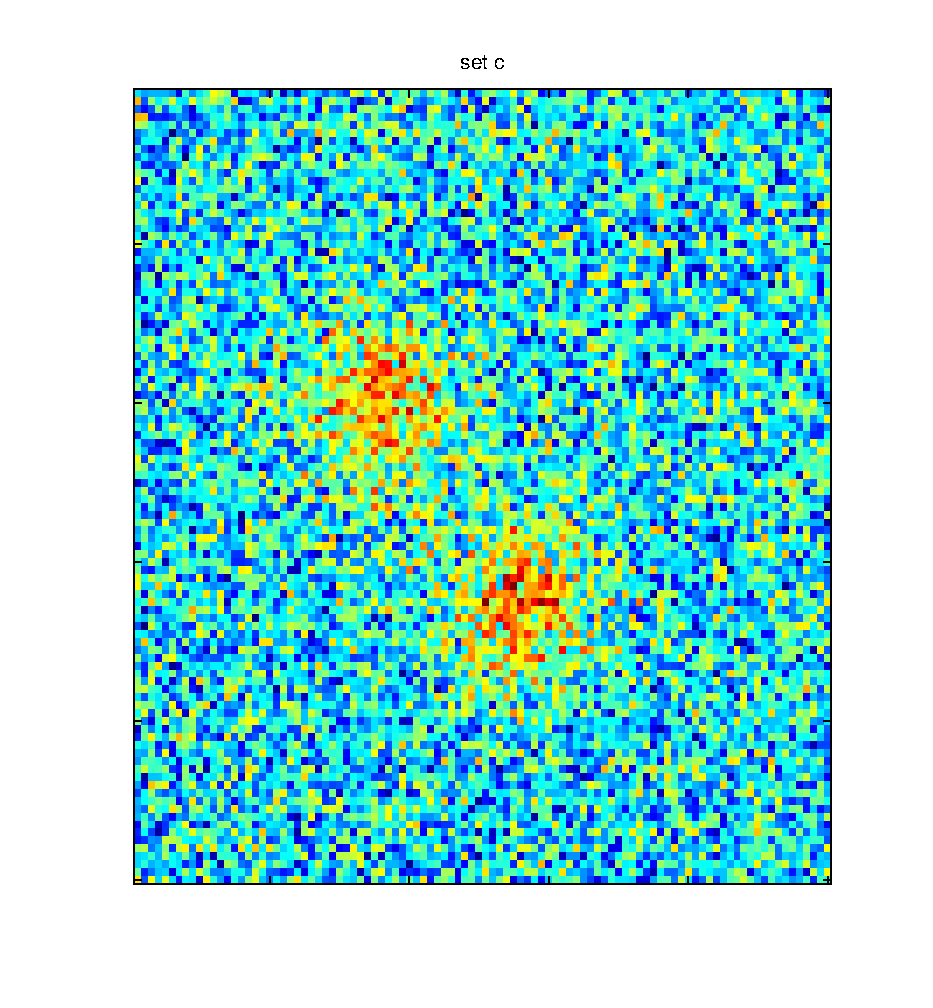
\includegraphics[width=1\linewidth]{figures/set_c.eps}
			\end{column}
		\end{columns}
	\end{frame}
	
	\begin{frame}
		\frametitle{Real World Data}
		\begin{columns}
			\begin{column}{.5\linewidth}
				But we probably are actually only getting something like this.

				How would we tackle this data set?

				Assume that we don't have known classes or groups.
			\end{column}
			\begin{column}{.5\linewidth}
				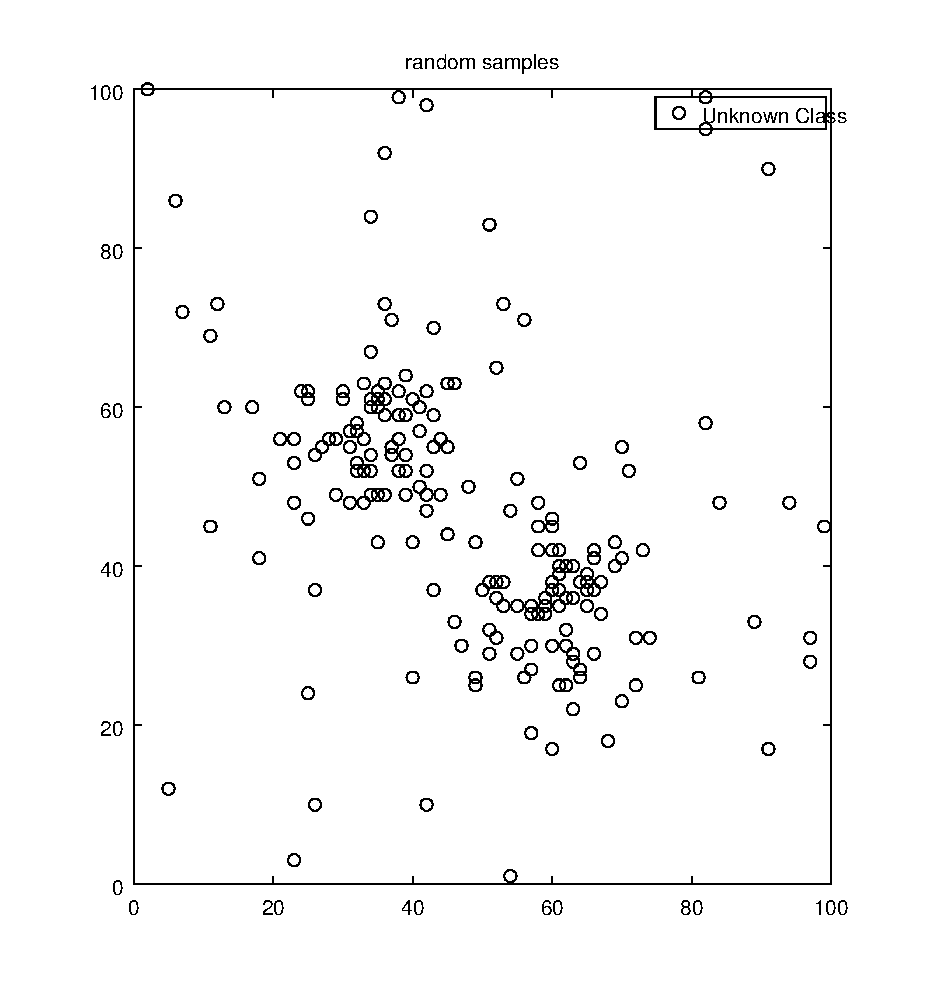
\includegraphics[width=1\linewidth]{figures/random_samples.eps}
			\end{column}
		\end{columns}
	\end{frame}

	\subsection{Linear Regression}
	\begin{frame}
		\frametitle{Linear Regression}
		\begin{columns}
			\begin{column}{.5\linewidth}
				We could regress it, with linear regression.

				This tries to relate the $y$ to the $x$.  Depending on $x$, we will try to predict the $y$ values.
			\end{column}
			\begin{column}{.5\linewidth}
				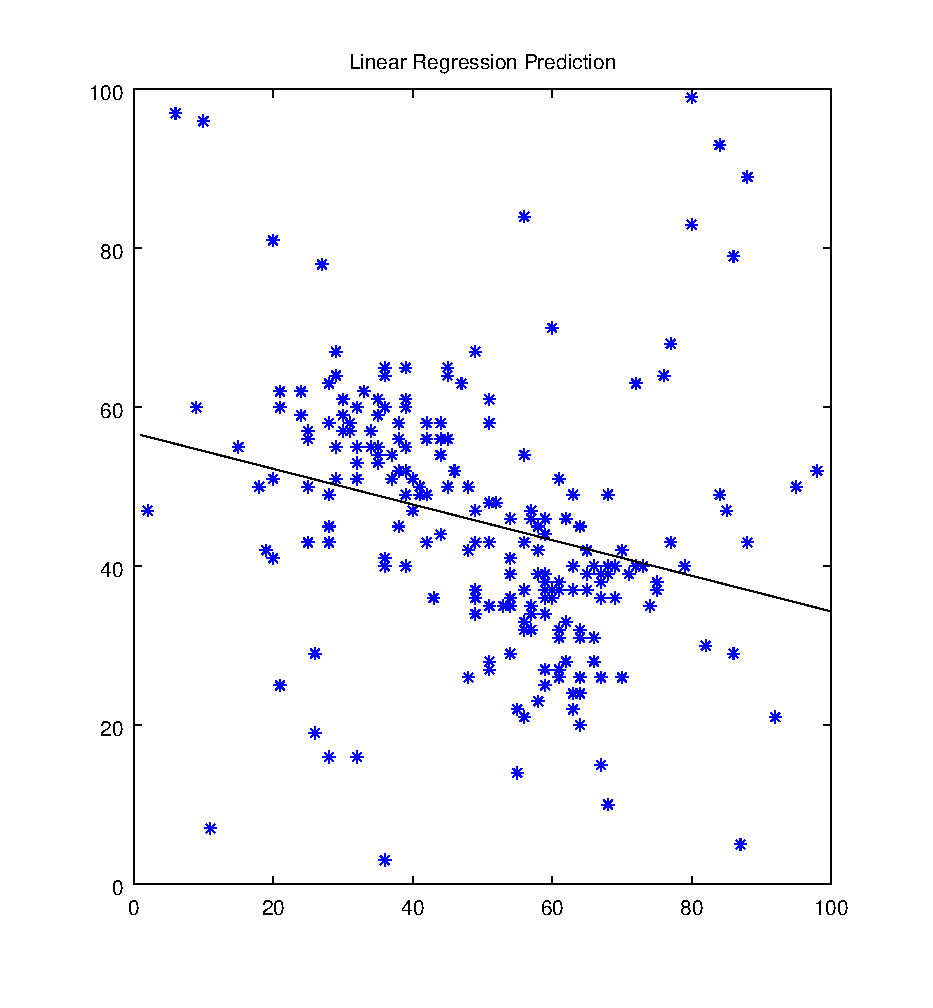
\includegraphics[width=1\linewidth]{figures/linear_regression.eps}
			\end{column}
		\end{columns}
	\end{frame}

	\subsection{Clusters}
	\begin{frame}
		\frametitle{Clusters}
		\begin{columns}
			\begin{column}{.5\linewidth}
				Or if we step back, we can see that this kind of looks like a cluster of data.

				Call it a cluster?

				But really it looks like there are two clusters there.
			\end{column}
			\begin{column}{.5\linewidth}
				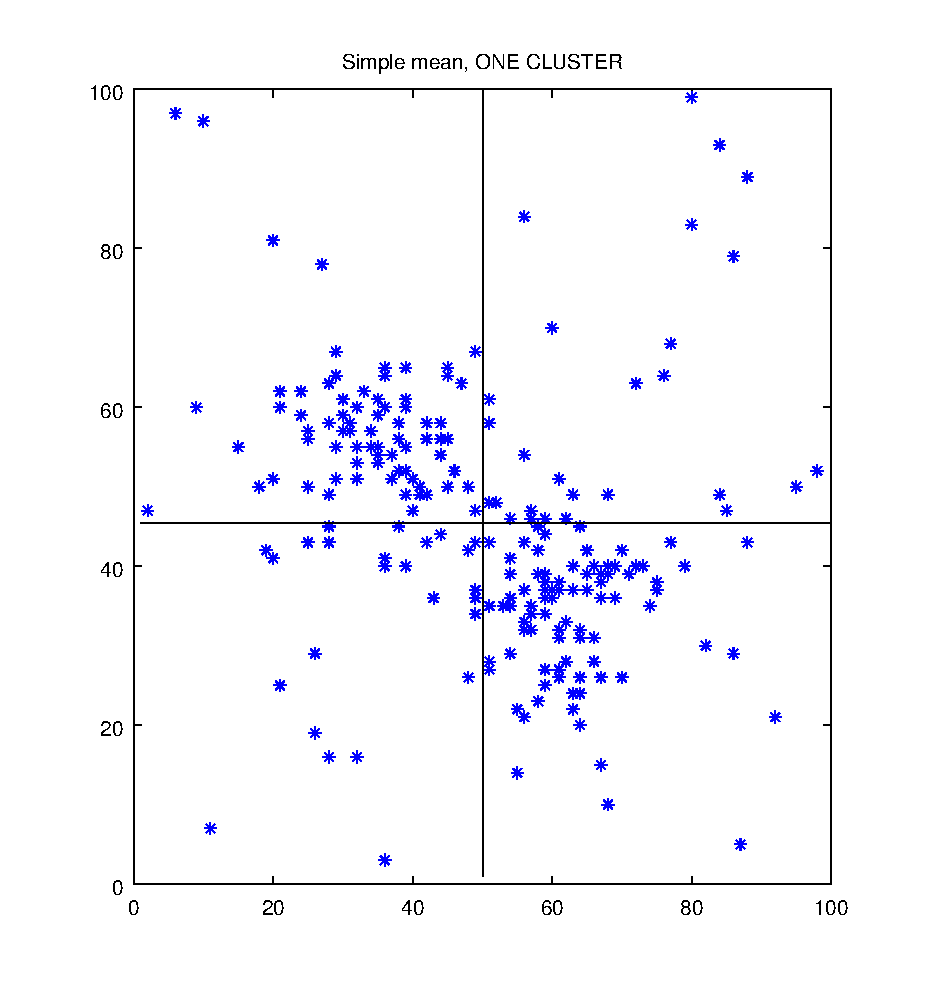
\includegraphics[width=1\linewidth]{figures/one_cluster.eps}
			\end{column}
		\end{columns}
	\end{frame}

\section{Classification}
	\subsection{K-Means}
	\begin{frame}
	\frametitle{K-Means}
		\begin{itemize}
			\item k-means is an unsupervised learning method
			\item nothing is known about classification of data points in the group
			\item we seek to identify groups that are similar
			\item what set of points has an affinity to others?
		\end{itemize}
	\end{frame}

	\begin{frame}
	\frametitle{K-Means How-To}
		\begin{enumerate}
			\item randomly sample N data points from the source set
			\item assign each of those to a cluster group
			\item while (data remains)
			\begin{enumerate}
				\item randomly select one point
				\item measure the distance to the centroids of the clusters\\(mean of $x$ and $y$ cluster points)
				\item assign to the closest cluster
				\item remove that data point and repeat
			\end{enumerate}
		\end{enumerate}
	\end{frame}

	\begin{frame}
		\frametitle{K-Means Step-by-Step}
		\begin{columns}
			\begin{column}{.5\linewidth}
				\begin{enumerate}
				\item Randomly selected 2 points.
				\item The magenta and the green points make up our two cluster groups.
				\item While data remains...
					\begin{enumerate}
					\item Randomly select a new point (blue dot with magenta and green lines connecting).
					\item Find the distance to the centroids ($+$).
					\item Assign to the closest.
					\item Remove that one and repeat.
					\end{enumerate}
				\end{enumerate}
				% Let's pause for a second... you and I might say that these magenta and green points live in the same cluster, right?

				% That's okay!  Let's run with it...
			\end{column}
			\begin{column}{.5\linewidth}
				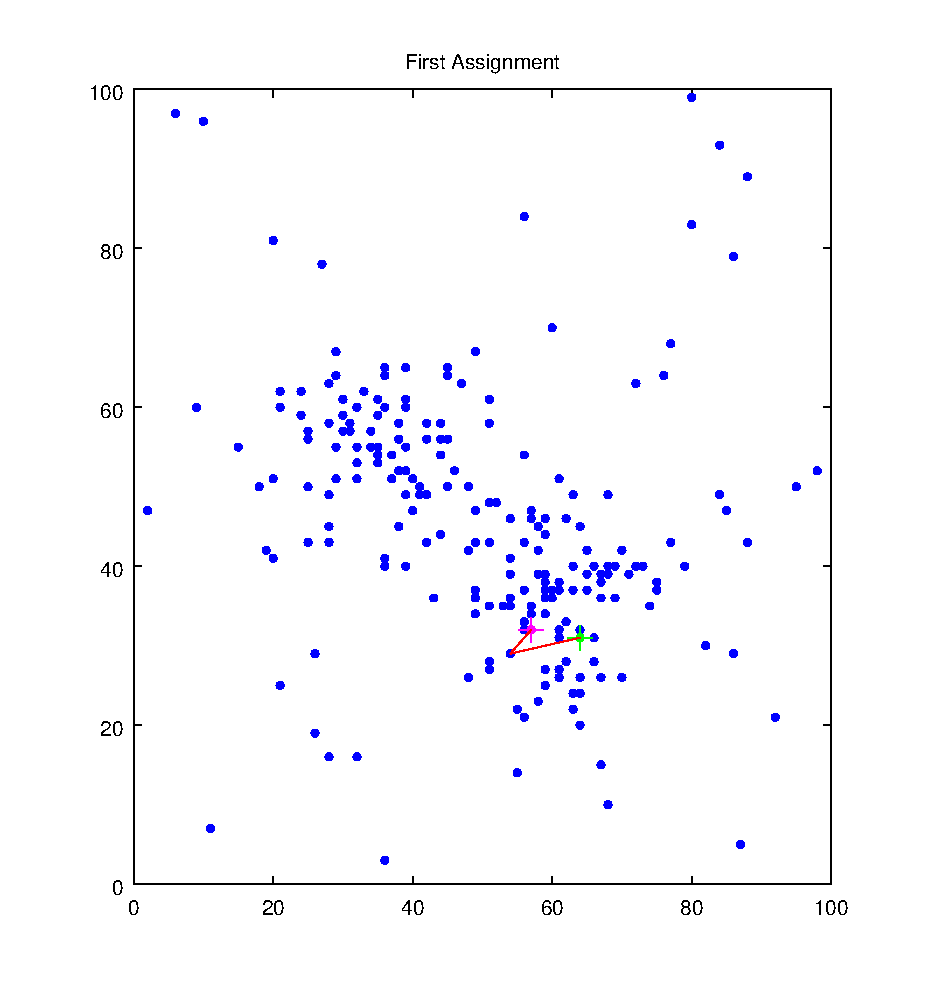
\includegraphics[width=1\linewidth]{figures/first_assignment.eps}
			\end{column}
		\end{columns}
	\end{frame}

		\begin{frame}
		\frametitle{K-Means Step-by-Step}
		\begin{columns}
			\begin{column}{.5\linewidth}
				% \begin{enumerate}
				% \item Randomly selected 2 points.
				% \item The magenta and the green points make up our two cluster groups.
				% \item While data remains...
				% 	\begin{enumerate}
				% 	\item Randomly select a new point (blue dot with magenta and green lines connecting).
				% 	\item Find the distance to the centroids ($+$).
				% 	\item Assign to the closest.
				% 	\item Remove that one and repeat.
				% 	\end{enumerate}
				% \end{enumerate}
				Let's pause for a second... you and I might say that these magenta and green points live in the same cluster, right?

				That's okay!  Let's run with it...
			\end{column}
			\begin{column}{.5\linewidth}
				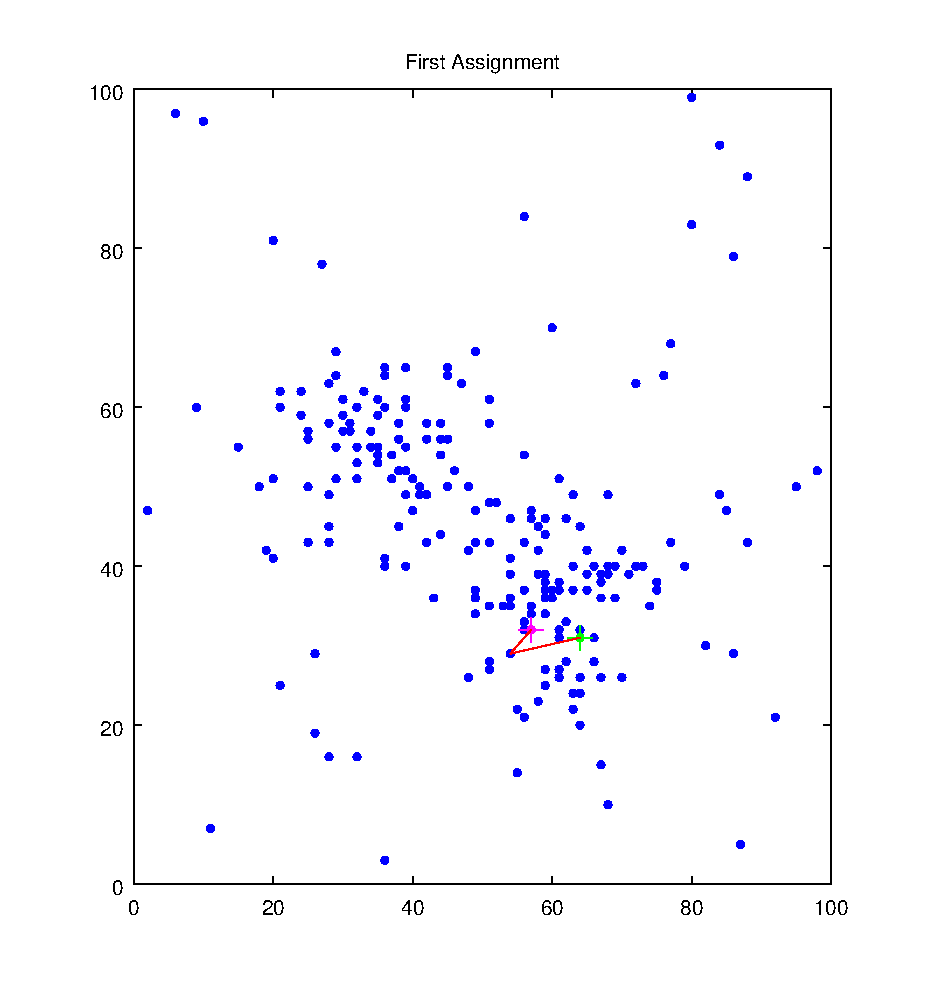
\includegraphics[width=1\linewidth]{figures/first_assignment.eps}
			\end{column}
		\end{columns}
	\end{frame}

	\begin{frame}
		\frametitle{K-Means Step-by-Step}
		\begin{columns}
			\begin{column}{.5\linewidth}
				\begin{enumerate}
				\item Randomly selected 2 points.
				\item The magenta and the green points make up our two cluster groups.
				\item While data remains...
					\begin{enumerate}
					\item Randomly select a new point (blue dot with magenta and green lines connecting).
					\item Find the distance to the centroids ($+$).
					\item Assign to the closest.
					\item Remove that one and repeat.
					\end{enumerate}
				\end{enumerate}
			\end{column}
			\begin{column}{.5\linewidth}
				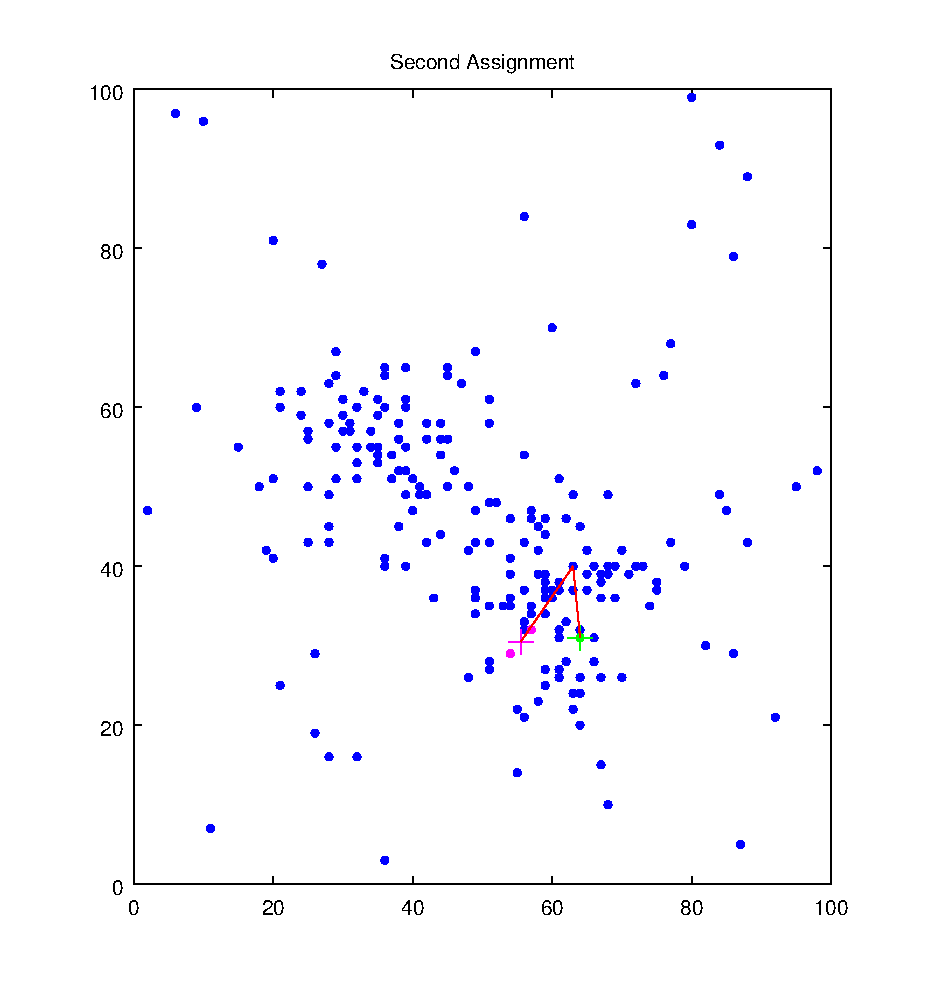
\includegraphics[width=1\linewidth]{figures/second_assignment.eps}
			\end{column}
		\end{columns}
	\end{frame}

	\begin{frame}
		\frametitle{K-Means Step-by-Step}
		\begin{columns}
			\begin{column}{.5\linewidth}
				\begin{enumerate}
				\item Randomly selected 2 points.
				\item The magenta and the green points make up our two cluster groups.
				\item While data remains...
					\begin{enumerate}
					\item Randomly select a new point (blue dot with magenta and green lines connecting).
					\item Find the distance to the centroids ($+$).
					\item Assign to the closest.
					\item Remove that one and repeat.
					\end{enumerate}
				\end{enumerate}
			\end{column}
			\begin{column}{.5\linewidth}
				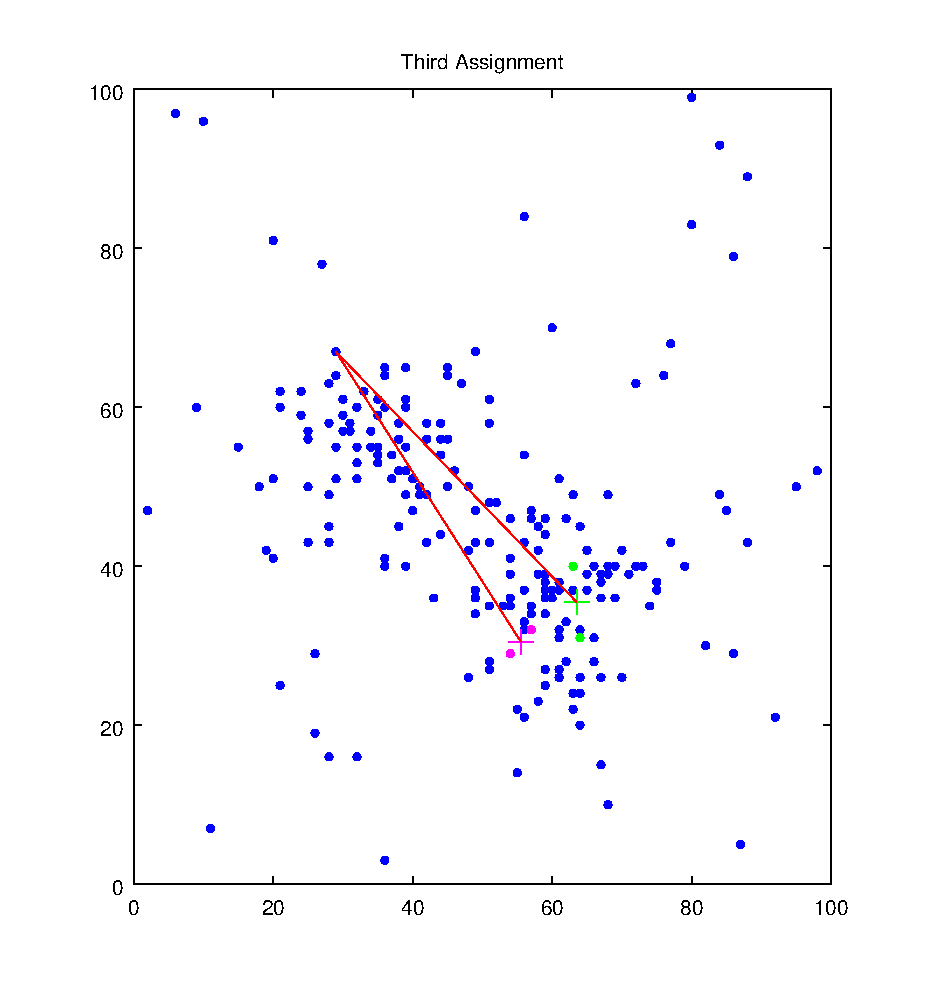
\includegraphics[width=1\linewidth]{figures/third_assignment.eps}
			\end{column}
		\end{columns}
	\end{frame}

	\begin{frame}
		\frametitle{K-Means Step-by-Step}
		\begin{columns}
			\begin{column}{.5\linewidth}
				\begin{enumerate}
				\item Randomly selected 2 points.
				\item The magenta and the green points make up our two cluster groups.
				\item While data remains...
					\begin{enumerate}
					\item Randomly select a new point (blue dot with magenta and green lines connecting).
					\item Find the distance to the centroids ($+$).
					\item Assign to the closest.
					\item Remove that one and repeat.
					\end{enumerate}
				\end{enumerate}
			\end{column}
			\begin{column}{.5\linewidth}
				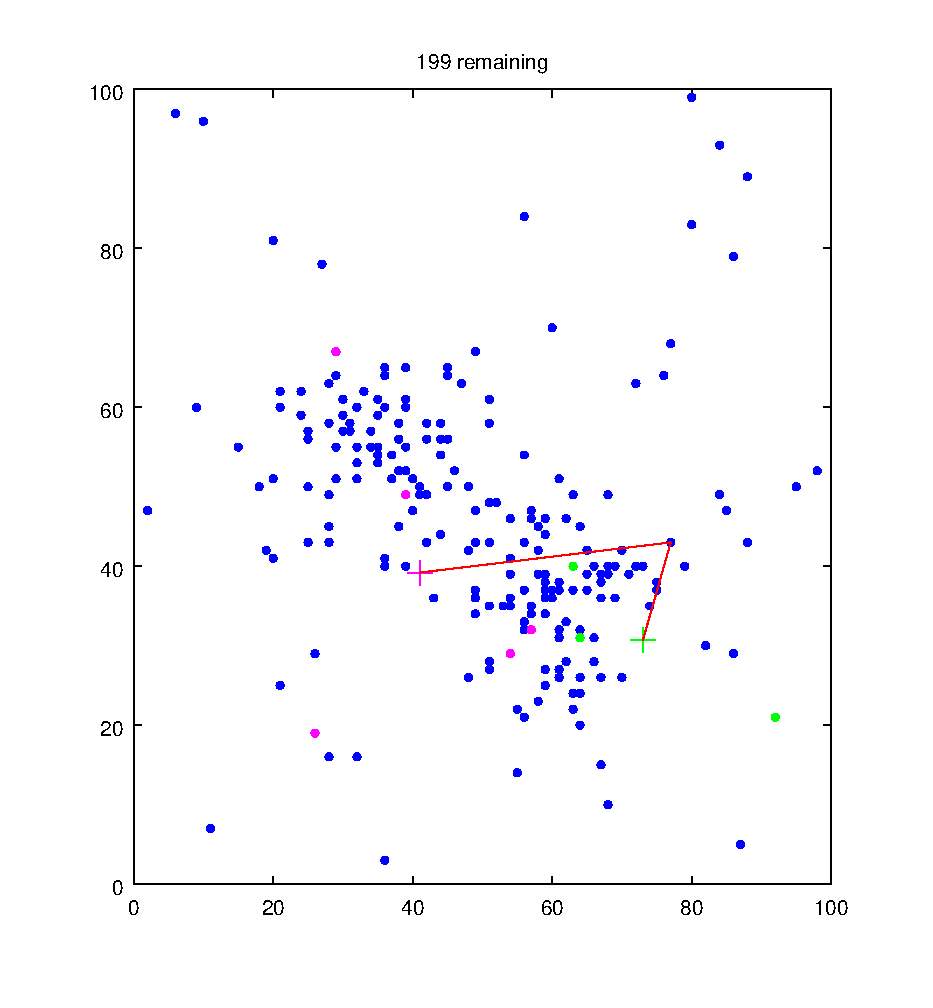
\includegraphics[width=1\linewidth]{figures/xstep_199.eps}
			\end{column}
		\end{columns}
	\end{frame}

	\begin{frame}
		\frametitle{K-Means Step-by-Step}
		\begin{columns}
			\begin{column}{.5\linewidth}
				\begin{enumerate}
				\item Randomly selected 2 points.
				\item The magenta and the green points make up our two cluster groups.
				\item While data remains...
					\begin{enumerate}
					\item Randomly select a new point (blue dot with magenta and green lines connecting).
					\item Find the distance to the centroids ($+$).
					\item Assign to the closest.
					\item Remove that one and repeat.
					\end{enumerate}
				\end{enumerate}
			\end{column}
			\begin{column}{.5\linewidth}
				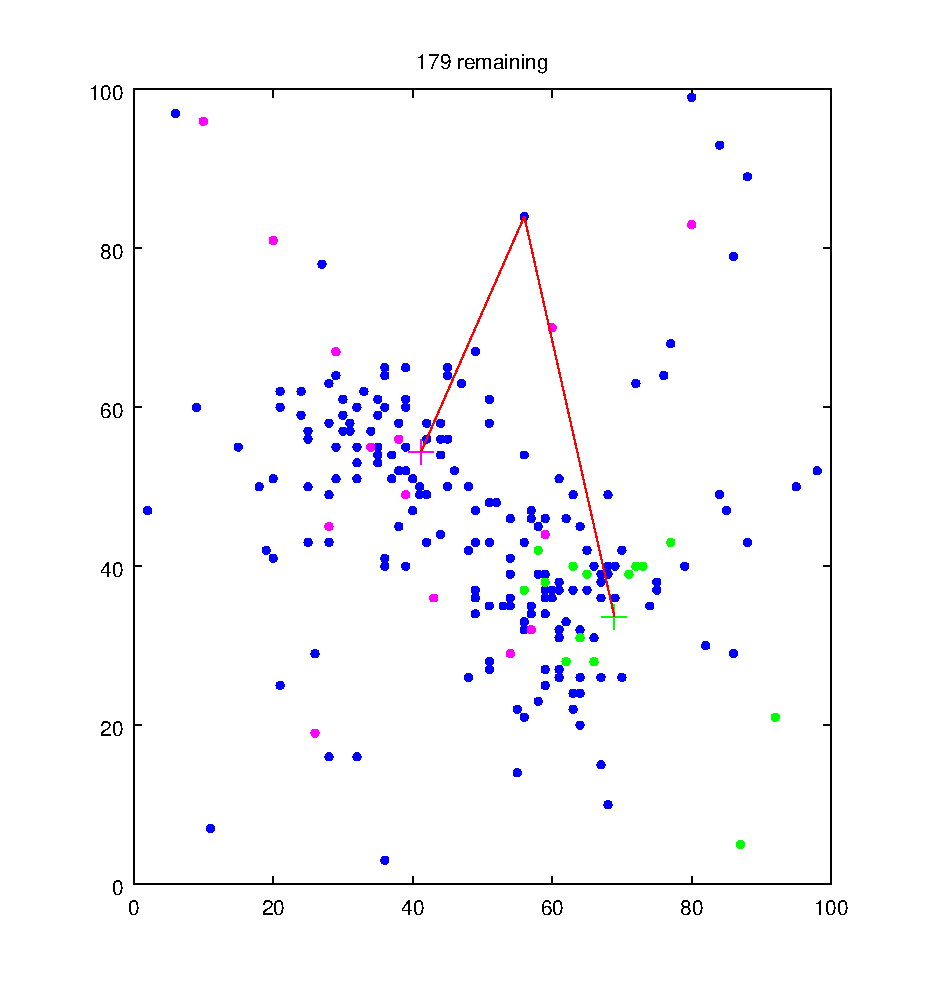
\includegraphics[width=1\linewidth]{figures/xstep_179.eps}
			\end{column}
		\end{columns}
	\end{frame}

	\begin{frame}
		\frametitle{K-Means Step-by-Step}
		\begin{columns}
			\begin{column}{.5\linewidth}
				\begin{enumerate}
				\item Randomly selected 2 points.
				\item The magenta and the green points make up our two cluster groups.
				\item While data remains...
					\begin{enumerate}
					\item Randomly select a new point (blue dot with magenta and green lines connecting).
					\item Find the distance to the centroids ($+$).
					\item Assign to the closest.
					\item Remove that one and repeat.
					\end{enumerate}
				\end{enumerate}
			\end{column}
			\begin{column}{.5\linewidth}
				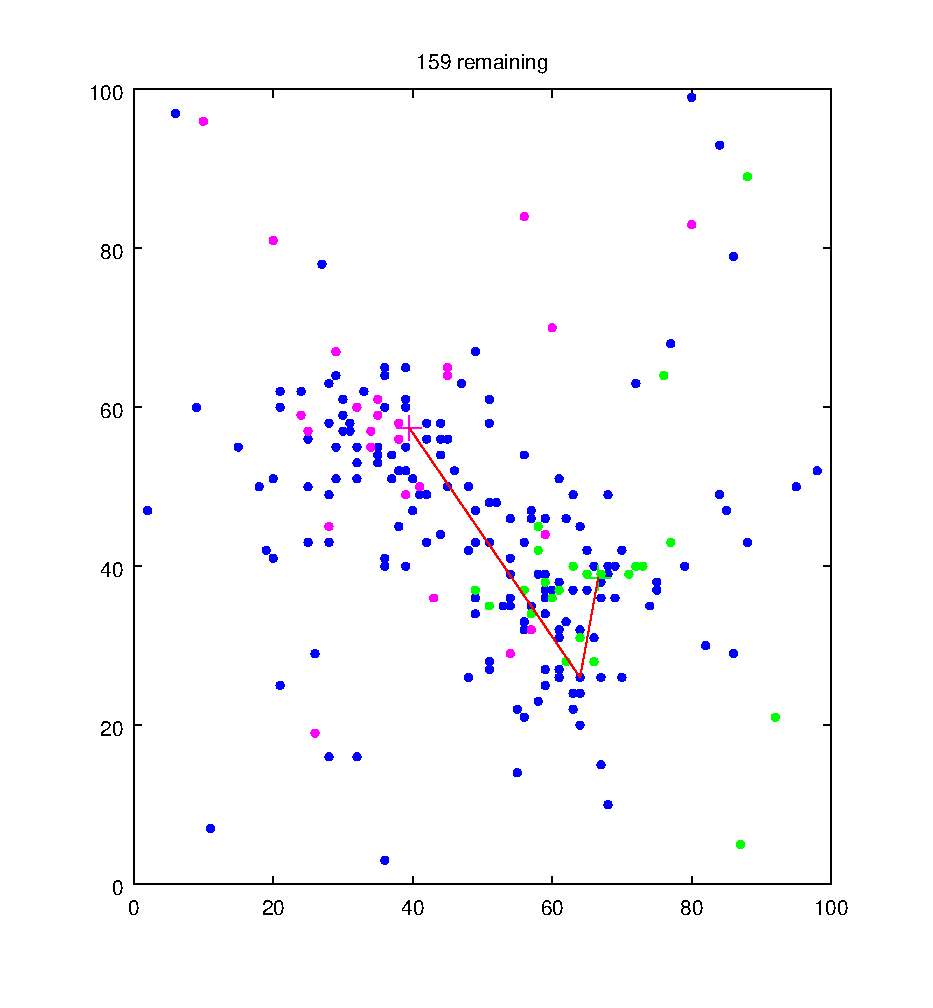
\includegraphics[width=1\linewidth]{figures/xstep_159.eps}
			\end{column}
		\end{columns}
	\end{frame}

	\begin{frame}
		\frametitle{K-Means Step-by-Step}
		\begin{columns}
			\begin{column}{.5\linewidth}
				\begin{enumerate}
				\item Randomly selected 2 points.
				\item The magenta and the green points make up our two cluster groups.
				\item While data remains...
					\begin{enumerate}
					\item Randomly select a new point (blue dot with magenta and green lines connecting).
					\item Find the distance to the centroids ($+$).
					\item Assign to the closest.
					\item Remove that one and repeat.
					\end{enumerate}
				\end{enumerate}
			\end{column}
			\begin{column}{.5\linewidth}
				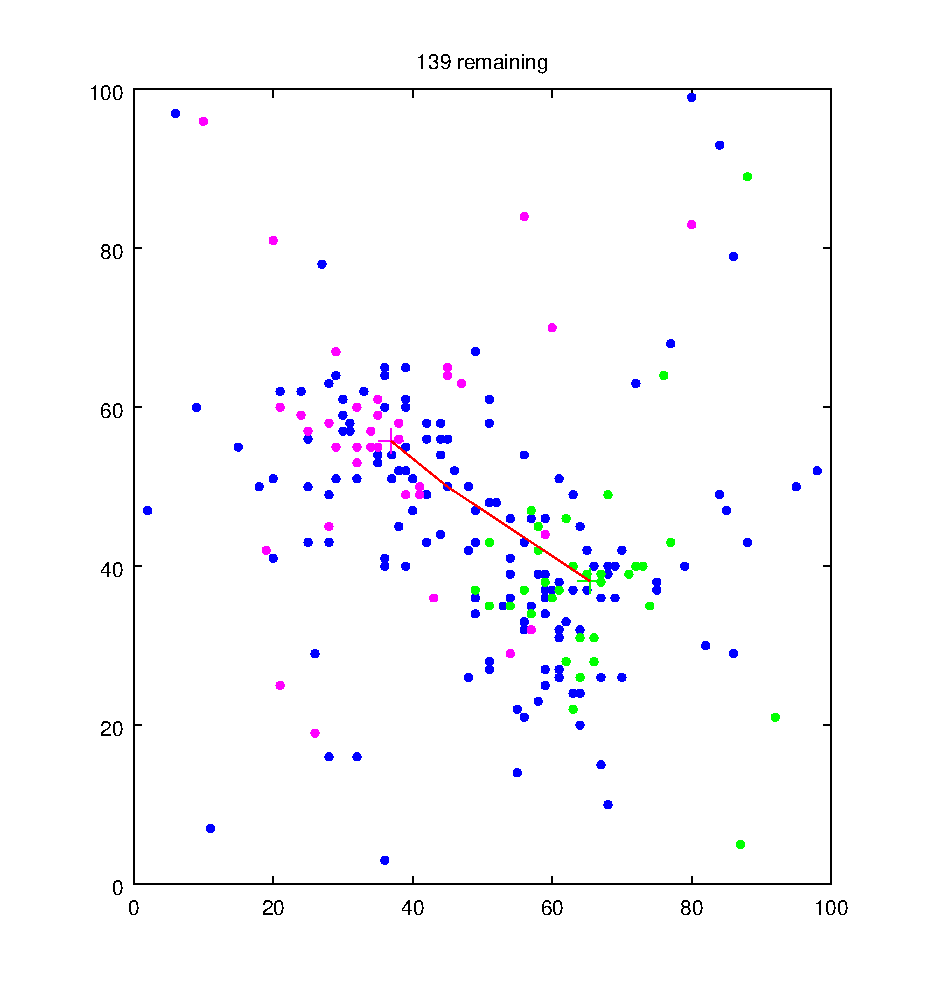
\includegraphics[width=1\linewidth]{figures/xstep_139.eps}
			\end{column}
		\end{columns}
	\end{frame}

	\begin{frame}
		\frametitle{K-Means Step-by-Step}
		\begin{columns}
			\begin{column}{.5\linewidth}
				\begin{enumerate}
				\item Randomly selected 2 points.
				\item The magenta and the green points make up our two cluster groups.
				\item While data remains...
					\begin{enumerate}
					\item Randomly select a new point (blue dot with magenta and green lines connecting).
					\item Find the distance to the centroids ($+$).
					\item Assign to the closest.
					\item Remove that one and repeat.
					\end{enumerate}
				\end{enumerate}
			\end{column}
			\begin{column}{.5\linewidth}
				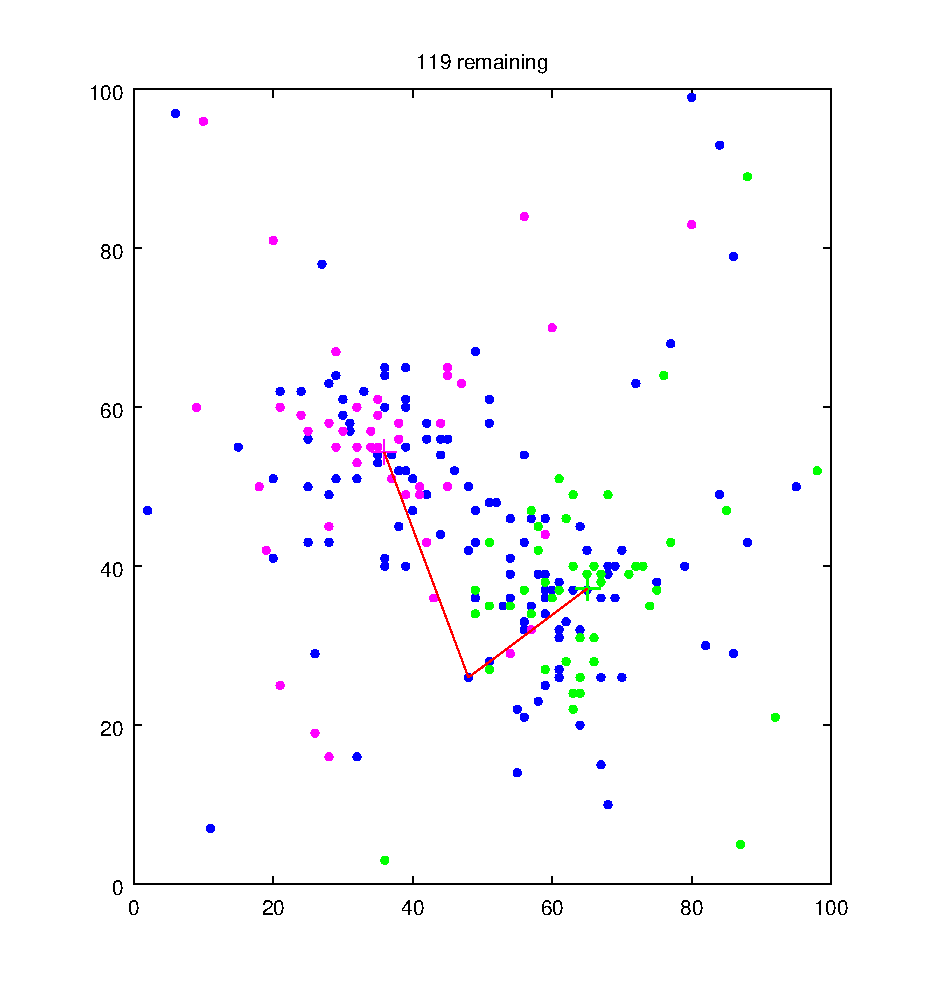
\includegraphics[width=1\linewidth]{figures/xstep_119.eps}
			\end{column}
		\end{columns}
	\end{frame}

	\begin{frame}
		\frametitle{K-Means Step-by-Step}
		\begin{columns}
			\begin{column}{.5\linewidth}
				\begin{enumerate}
				\item Randomly selected 2 points.
				\item The magenta and the green points make up our two cluster groups.
				\item While data remains...
					\begin{enumerate}
					\item Randomly select a new point (blue dot with magenta and green lines connecting).
					\item Find the distance to the centroids ($+$).
					\item Assign to the closest.
					\item Remove that one and repeat.
					\end{enumerate}
				\end{enumerate}
			\end{column}
			\begin{column}{.5\linewidth}
				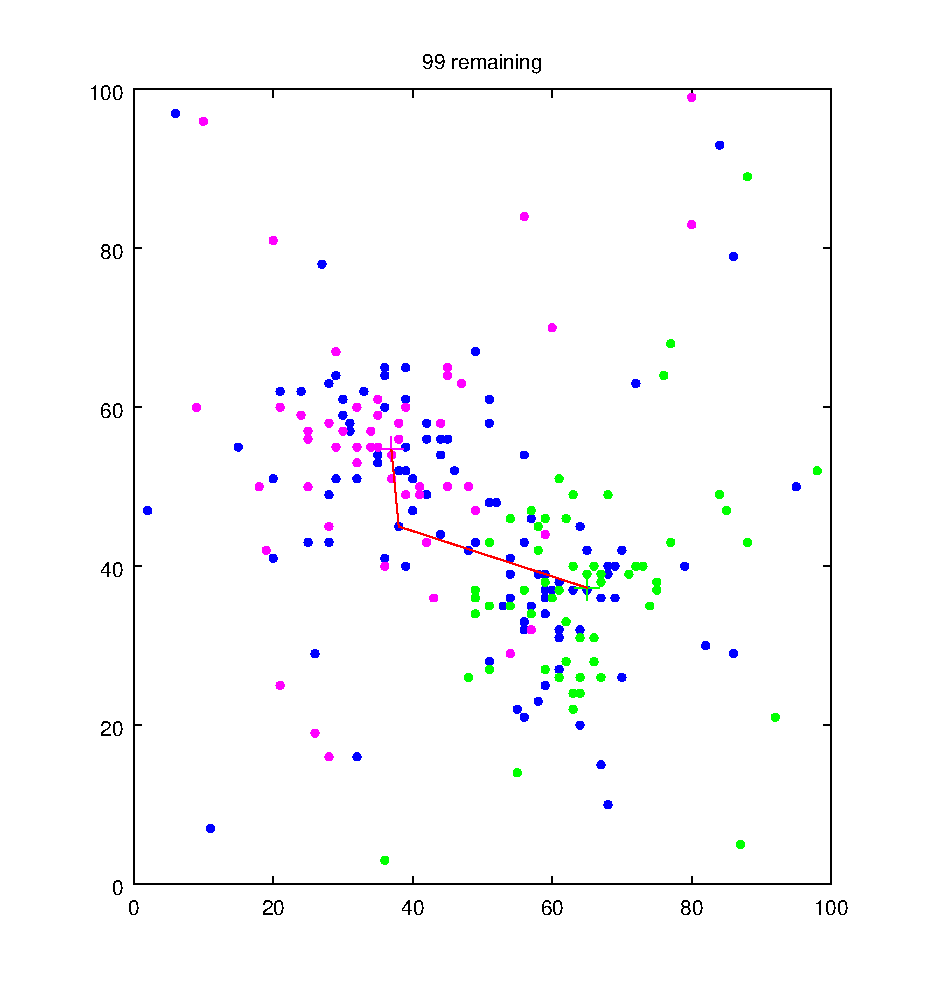
\includegraphics[width=1\linewidth]{figures/xstep_99.eps}
			\end{column}
		\end{columns}
	\end{frame}

	\begin{frame}
		\frametitle{K-Means Step-by-Step}
		\begin{columns}
			\begin{column}{.5\linewidth}
				\begin{enumerate}
				\item Randomly selected 2 points.
				\item The magenta and the green points make up our two cluster groups.
				\item While data remains...
					\begin{enumerate}
					\item Randomly select a new point (blue dot with magenta and green lines connecting).
					\item Find the distance to the centroids ($+$).
					\item Assign to the closest.
					\item Remove that one and repeat.
					\end{enumerate}
				\end{enumerate}
			\end{column}
			\begin{column}{.5\linewidth}
				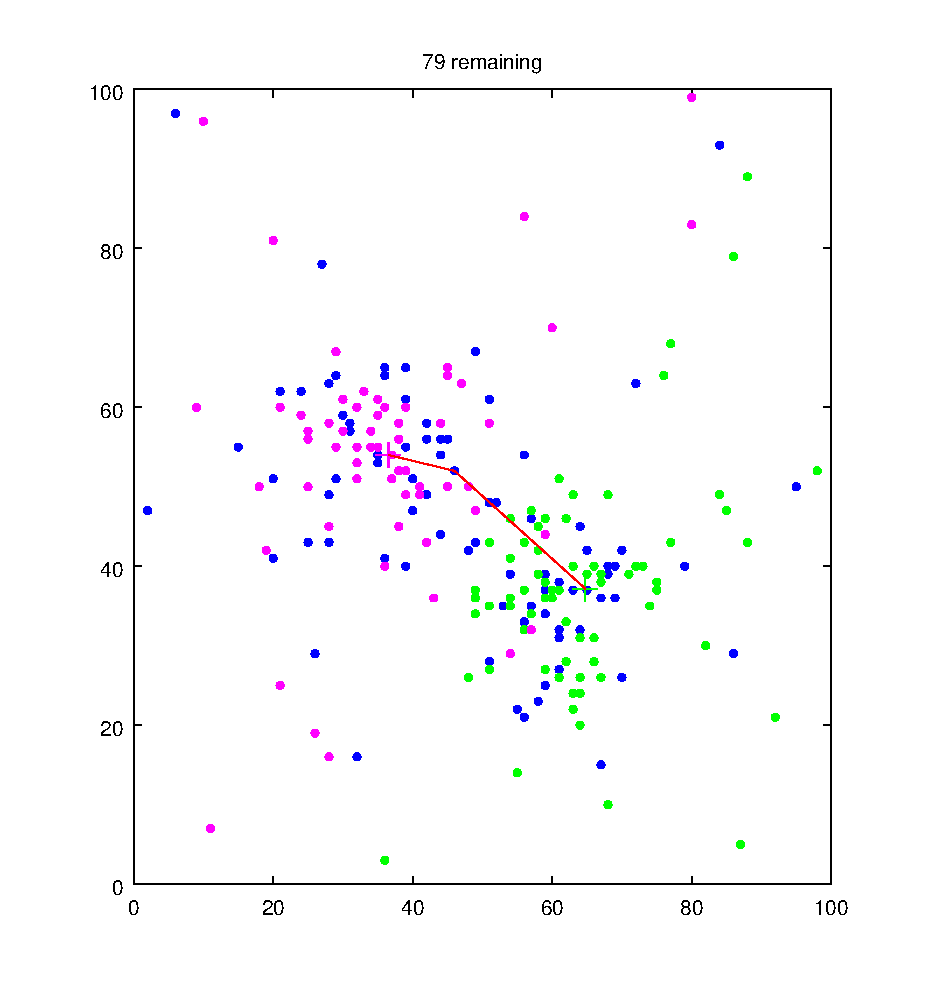
\includegraphics[width=1\linewidth]{figures/xstep_79.eps}
			\end{column}
		\end{columns}
	\end{frame}

	\begin{frame}
		\frametitle{K-Means Step-by-Step}
		\begin{columns}
			\begin{column}{.5\linewidth}
				\begin{enumerate}
				\item Randomly selected 2 points.
				\item The magenta and the green points make up our two cluster groups.
				\item While data remains...
					\begin{enumerate}
					\item Randomly select a new point (blue dot with magenta and green lines connecting).
					\item Find the distance to the centroids ($+$).
					\item Assign to the closest.
					\item Remove that one and repeat.
					\end{enumerate}
				\end{enumerate}
			\end{column}
			\begin{column}{.5\linewidth}
				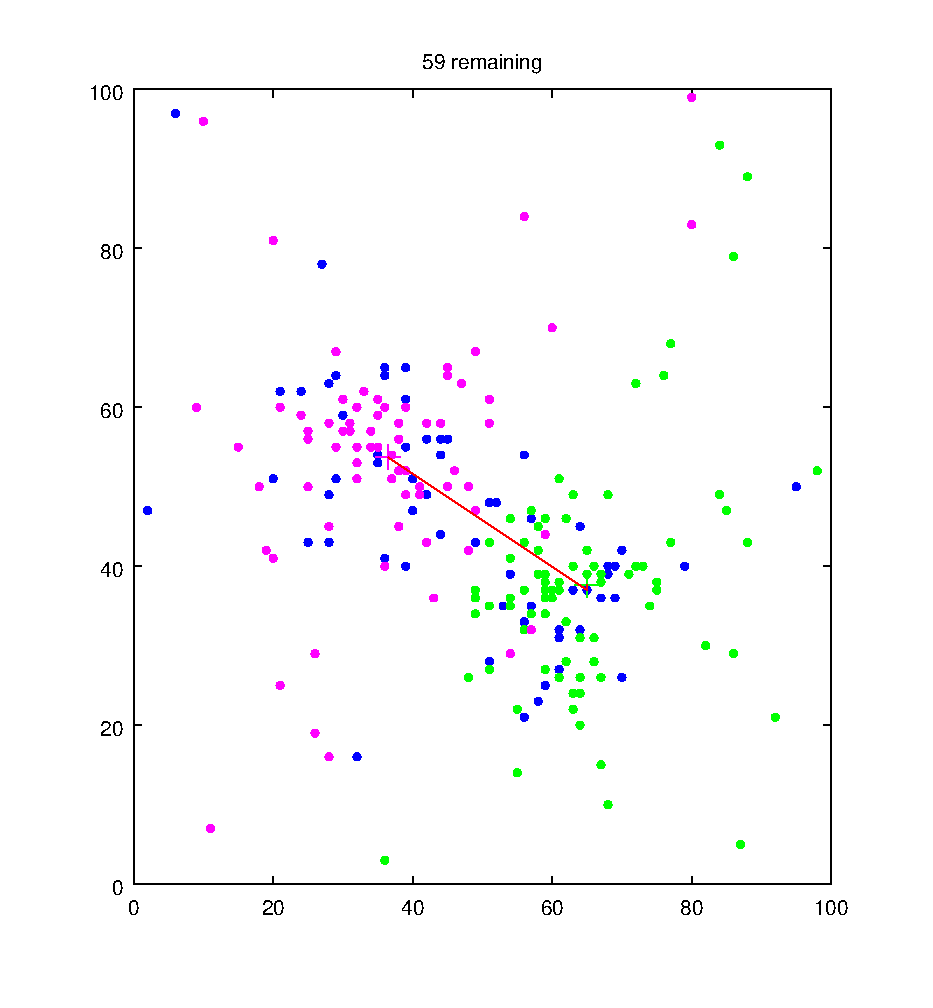
\includegraphics[width=1\linewidth]{figures/xstep_59.eps}
			\end{column}
		\end{columns}
	\end{frame}

	\begin{frame}
		\frametitle{K-Means Step-by-Step}
		\begin{columns}
			\begin{column}{.5\linewidth}
				\begin{enumerate}
				\item Randomly selected 2 points.
				\item The magenta and the green points make up our two cluster groups.
				\item While data remains...
					\begin{enumerate}
					\item Randomly select a new point (blue dot with magenta and green lines connecting).
					\item Find the distance to the centroids ($+$).
					\item Assign to the closest.
					\item Remove that one and repeat.
					\end{enumerate}
				\end{enumerate}
			\end{column}
			\begin{column}{.5\linewidth}
				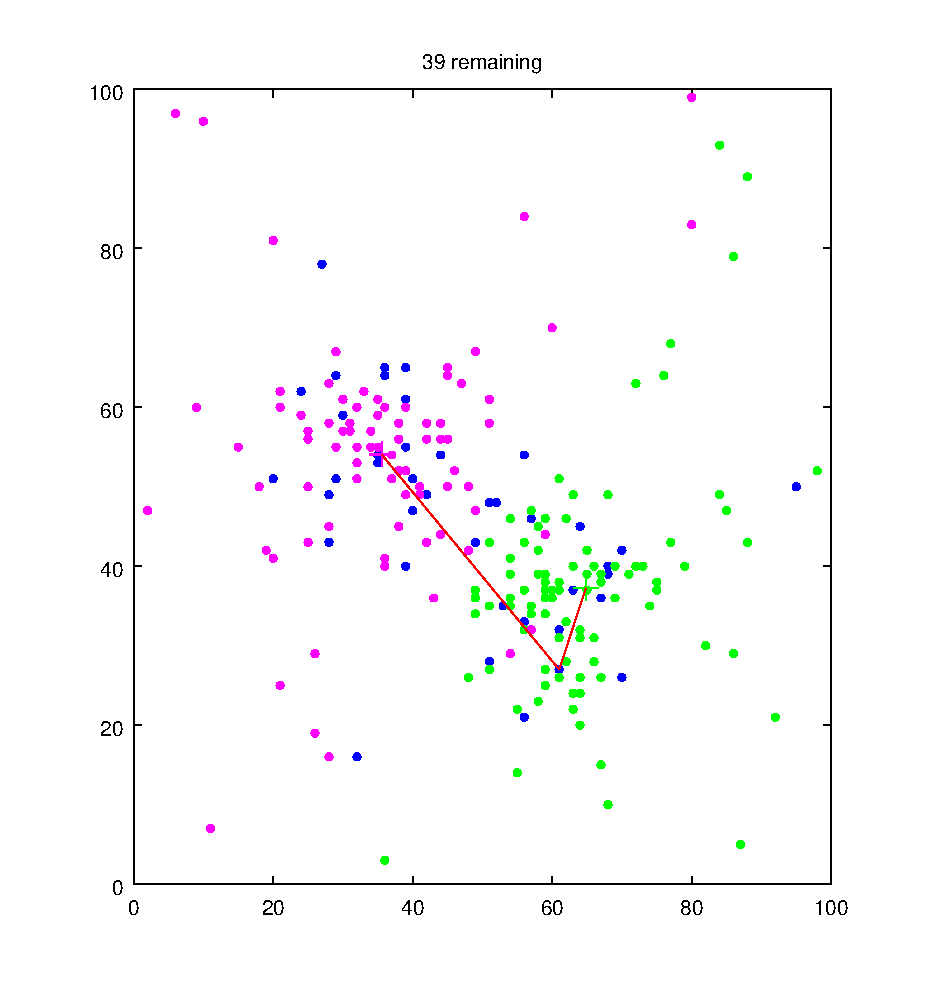
\includegraphics[width=1\linewidth]{figures/xstep_39.eps}
			\end{column}
		\end{columns}
	\end{frame}

	\begin{frame}
		\frametitle{K-Means Step-by-Step}
		\begin{columns}
			\begin{column}{.5\linewidth}
				\begin{enumerate}
				\item Randomly selected 2 points.
				\item The magenta and the green points make up our two cluster groups.
				\item While data remains...
					\begin{enumerate}
					\item Randomly select a new point (blue dot with magenta and green lines connecting).
					\item Find the distance to the centroids ($+$).
					\item Assign to the closest.
					\item Remove that one and repeat.
					\end{enumerate}
				\end{enumerate}
			\end{column}
			\begin{column}{.5\linewidth}
				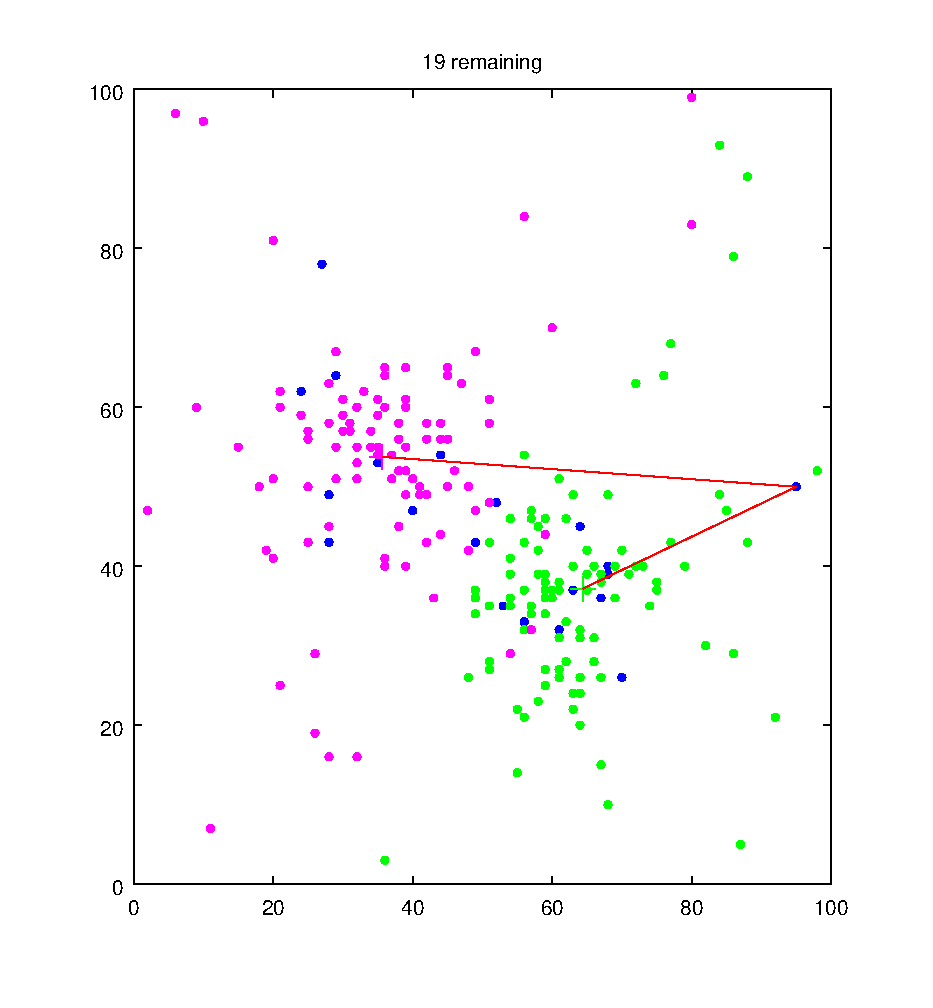
\includegraphics[width=1\linewidth]{figures/xstep_19.eps}
			\end{column}
		\end{columns}
	\end{frame}

	\begin{frame}
		\frametitle{K-Means Step-by-Step}
		\begin{columns}
			\begin{column}{.5\linewidth}
				\begin{enumerate}
				\item Randomly selected 2 points.
				\item The magenta and the green points make up our two cluster groups.
				\item While data remains...
					\begin{enumerate}
					\item Randomly select a new point (blue dot with magenta and green lines connecting).
					\item Find the distance to the centroids ($+$).
					\item Assign to the closest.
					\item Remove that one and repeat.
					\end{enumerate}
				\end{enumerate}
			\end{column}
			\begin{column}{.5\linewidth}
				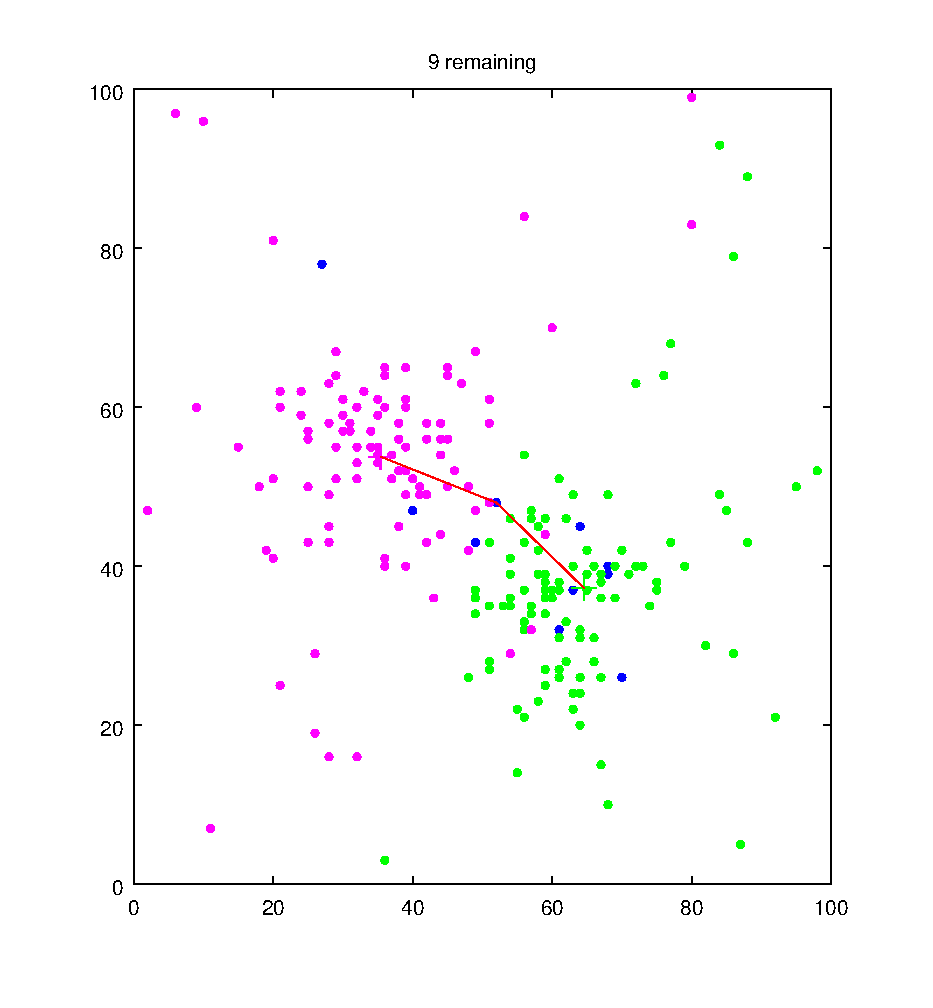
\includegraphics[width=1\linewidth]{figures/xstep_9.eps}
			\end{column}
		\end{columns}
	\end{frame}

	\begin{frame}
		\frametitle{K-Means Step-by-Step}
		\begin{columns}
			\begin{column}{.5\linewidth}
				\begin{enumerate}
				\item Randomly selected 2 points.
				\item The magenta and the green points make up our two cluster groups.
				\item While data remains...
					\begin{enumerate}
						\item Randomly select a new point (blue dot with magenta and green lines connecting).
						\item Find the distance to the centroids ($+$).
						\item Assign to the closest.
						\item Remove that one and repeat.
					\end{enumerate}
				\end{enumerate}
			\end{column}
			\begin{column}{.5\linewidth}
				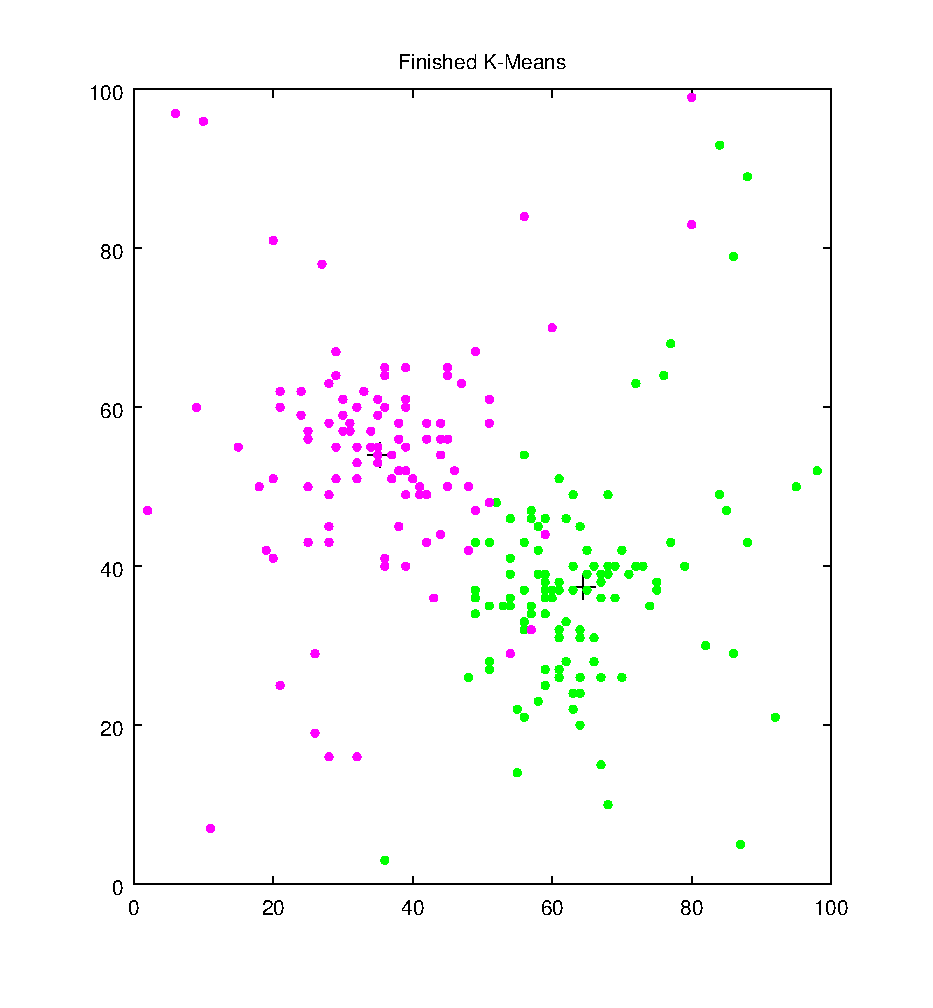
\includegraphics[width=1\linewidth]{figures/kmeans_done.eps}
			\end{column}
		\end{columns}
	\end{frame}

	\begin{frame}
		\frametitle{K-Means Step-by-Step}
		\begin{columns}
			\begin{column}{.5\linewidth}
				We have pulled them apart!

				Yes, some magenta dot live inside of the bounds of the green, and vise-versa... why?
			\end{column}
			\begin{column}{.5\linewidth}
				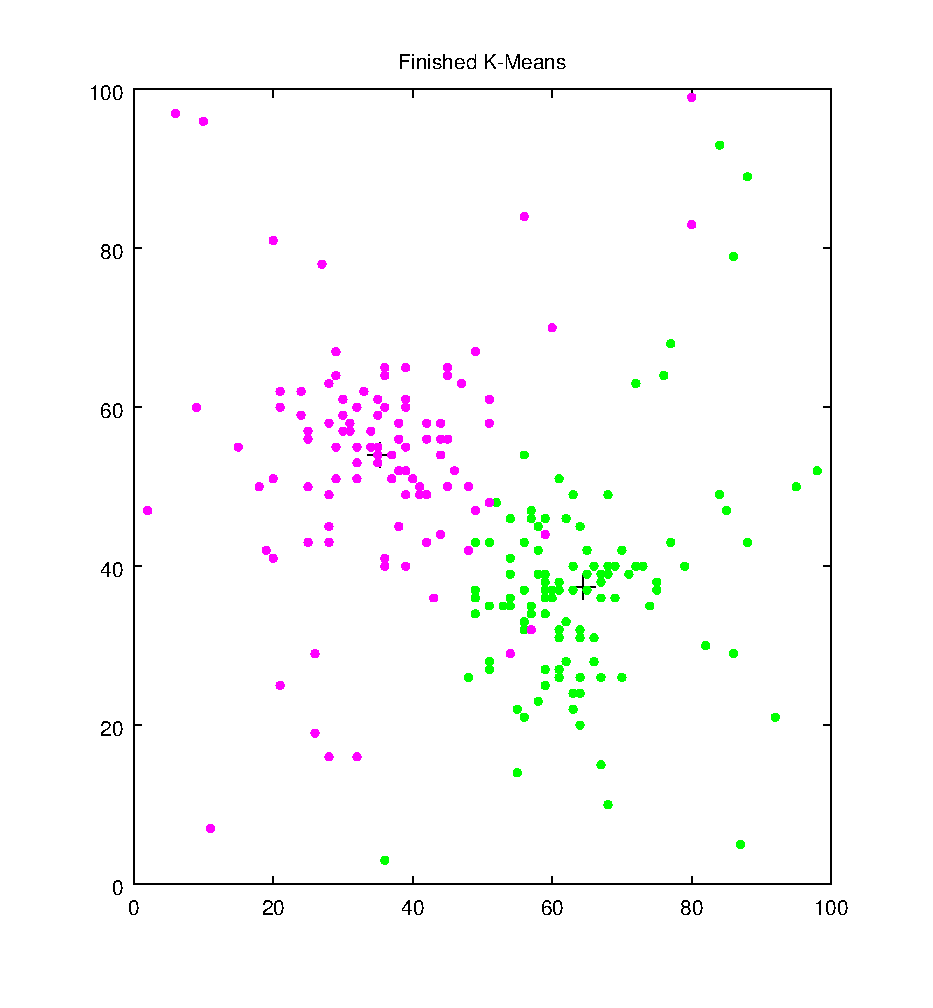
\includegraphics[width=1\linewidth]{figures/kmeans_done.eps}
			\end{column}
		\end{columns}
	\end{frame}

	\begin{frame}
		\frametitle{K-Means Step-by-Step}
		\begin{columns}
			\begin{column}{.5\linewidth}
				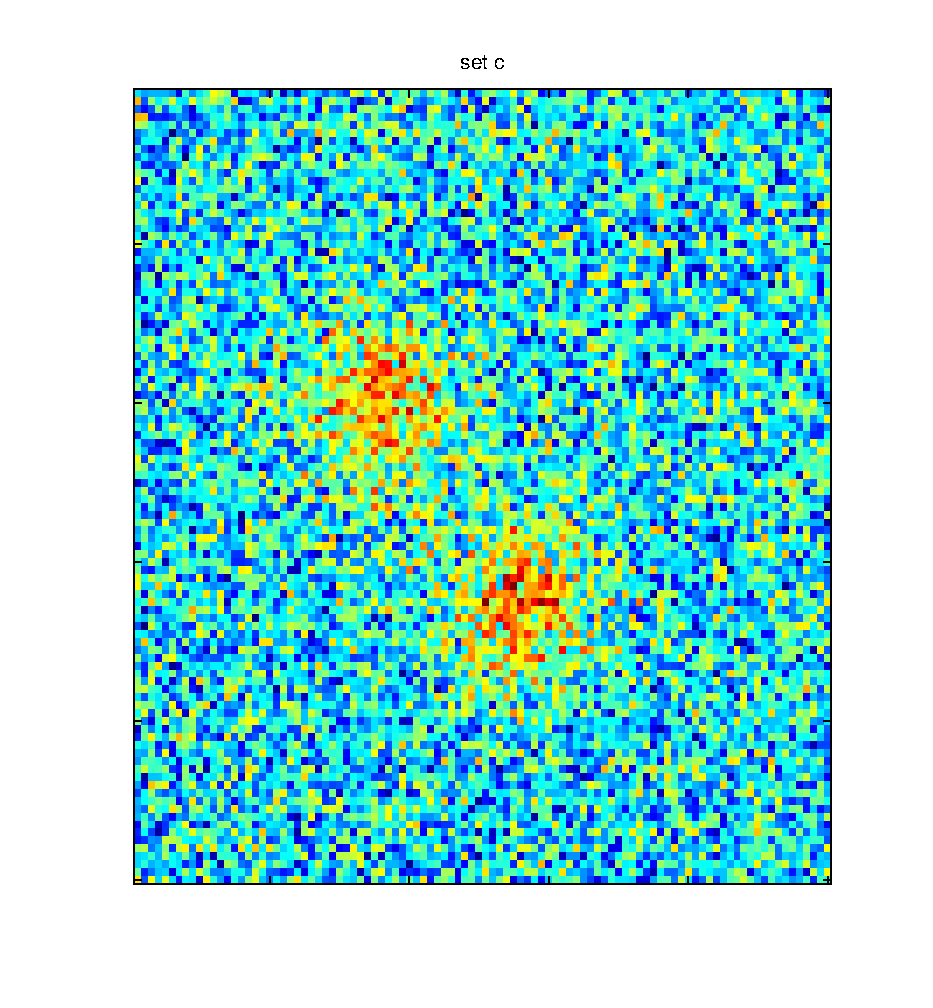
\includegraphics[width=1\linewidth]{figures/set_c.eps}
			\end{column}
			\begin{column}{.5\linewidth}
				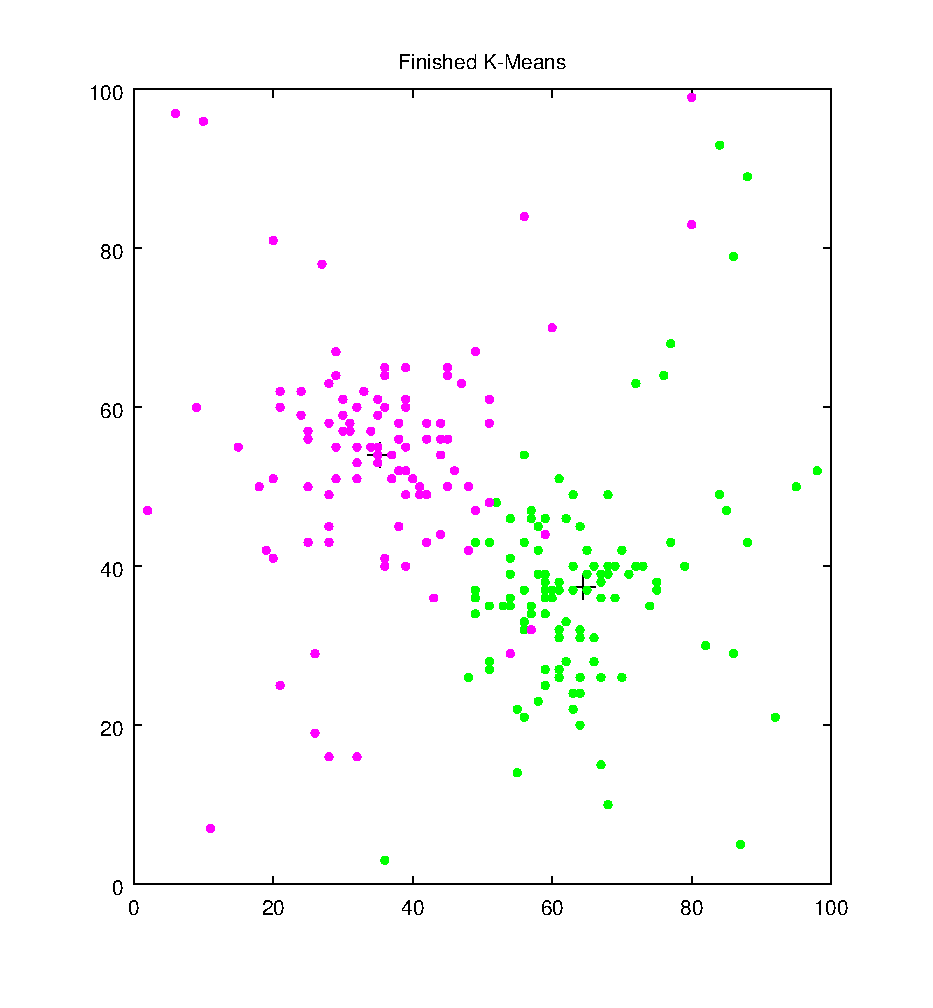
\includegraphics[width=1\linewidth]{figures/kmeans_done.eps}
			\end{column}
		\end{columns}
	\end{frame}

	\begin{frame}
		\frametitle{K-Means Step-by-Step}
		\begin{columns}
			\begin{column}{.5\linewidth}
				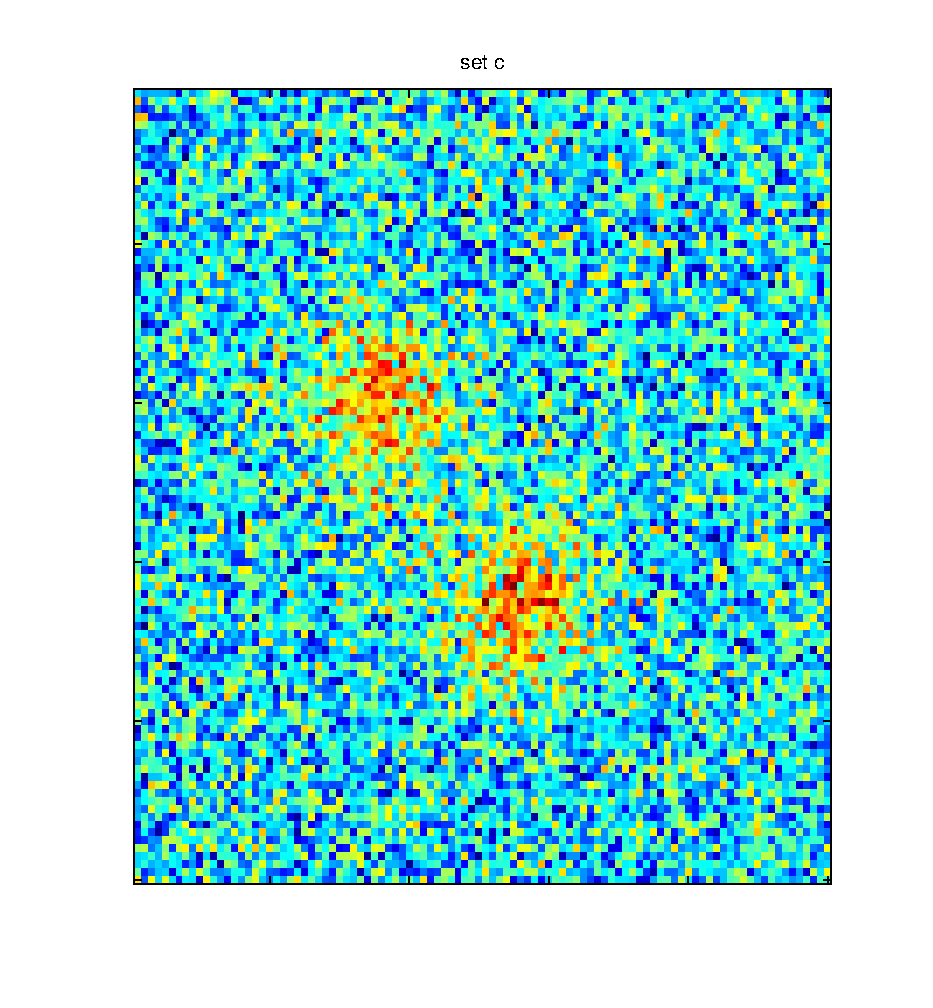
\includegraphics[width=1\linewidth]{figures/set_c.eps}
			\end{column}
			\begin{column}{.5\linewidth}
				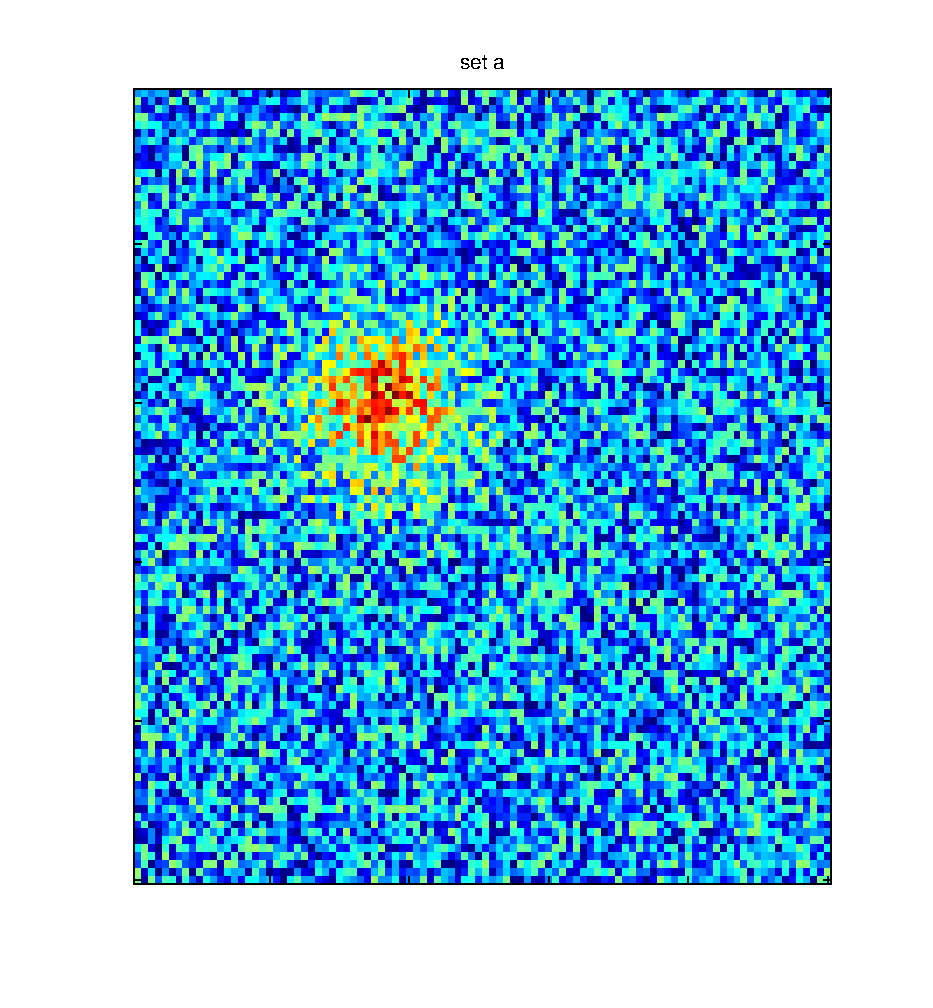
\includegraphics[width=.45\linewidth]{figures/set_a.eps}
				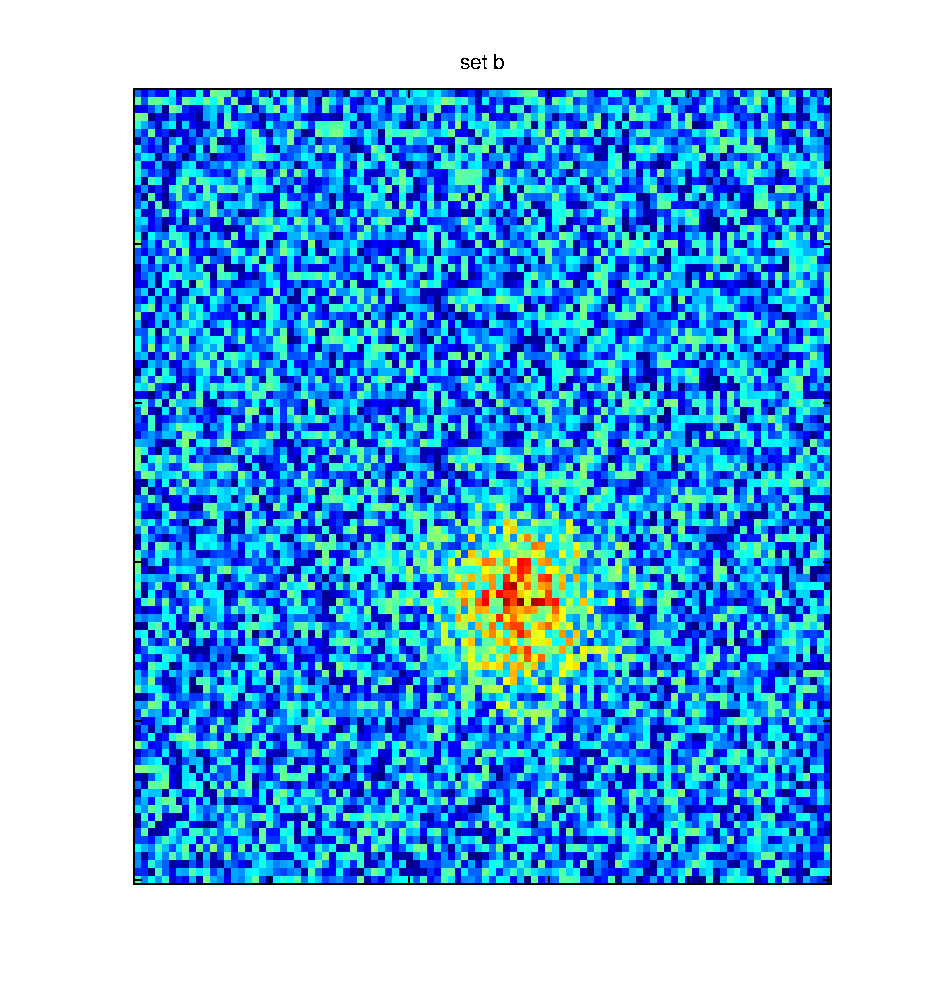
\includegraphics[width=.45\linewidth]{figures/set_b.eps}\\
				These might be two different datasets, that are clustered near each other.

				Could there be more? (2, 100, 200?)

				What might be some of the problems with k-means? (and the fix?)

				What are some advantages of k-means?

				% We can use this to find dividing lines between the data.
			\end{column}
		\end{columns}
	\end{frame}

	\begin{frame}
	\frametitle{K-Means Recap}
		\begin{itemize}
			\item For some new data points, consider what cluster centroid it is closest to, for assignment
			\item k-means is an unsupervised learning method
			\item nothing is known about classification of data points in the group
			\item we seek to identify groups that are similar
		\end{itemize}
	\end{frame}

	\subsection{K-Nearest-Neighbors}
	\begin{frame}
	\frametitle{K-Nearest-Neighbors (KNN)}
		\begin{columns}
			\begin{column}{.5\linewidth}
				Suppose we have labels...

				This could be Y/N, or Type 1, 2, 3, etc.

				We have assigned some red, and some blue.

				Oh, and this is that same dataset!
			\end{column}
			\begin{column}{.5\linewidth}
				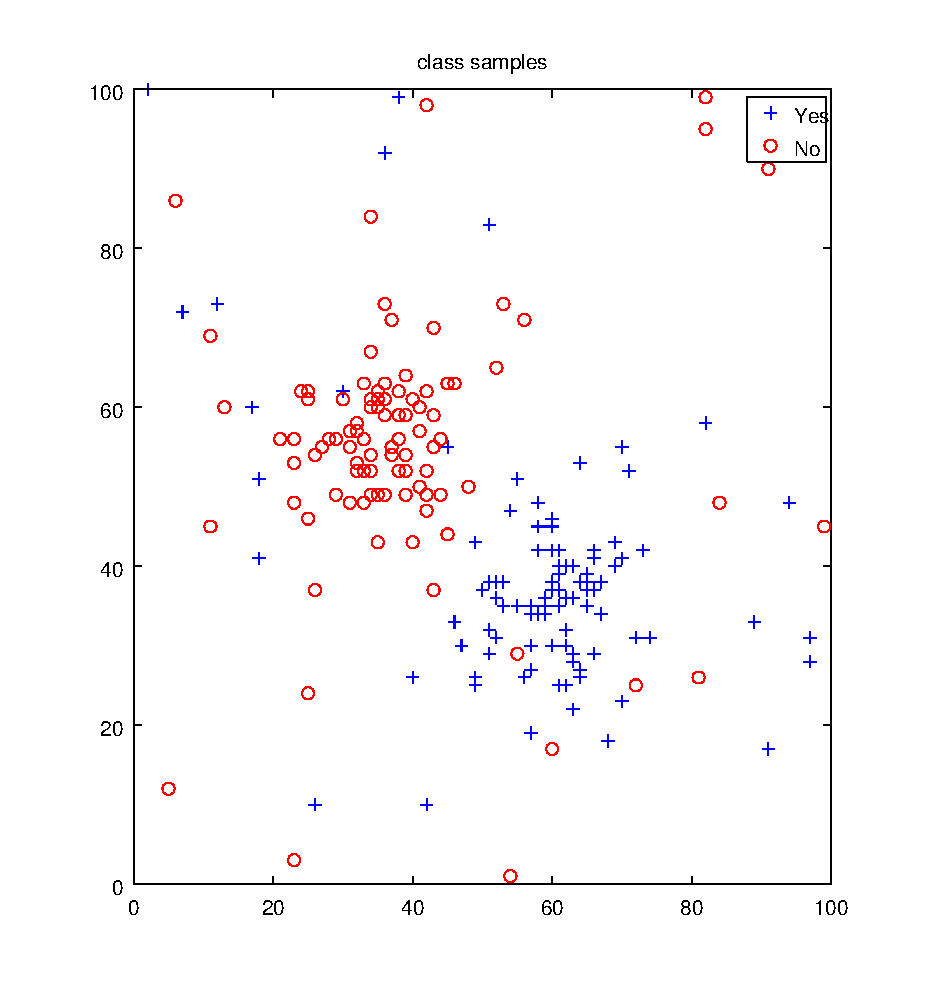
\includegraphics[width=1\linewidth]{figures/class_samples.eps}
			\end{column}
		\end{columns}
	\end{frame}

	\begin{frame}
	\frametitle{K-Nearest-Neighbors (KNN)}
		\begin{itemize}
			\item This time, assignment is decided on the N closest data points.
			\item Identify what the distribution of those data point classifications.  This is a vote!
			\item Supervised learning, as you're using the classification of other data to determine the classification of the new data points.
		\end{itemize}
	\end{frame}

	\begin{frame}
	\frametitle{KNN How-To}
		\begin{enumerate}
			\item For some point, select the N closest other data points.
			\item Find the classification with the highest {\em observed} probability for this set.
		\end{enumerate}
	\end{frame}

	\begin{frame}
	\frametitle{KNN How-To}
		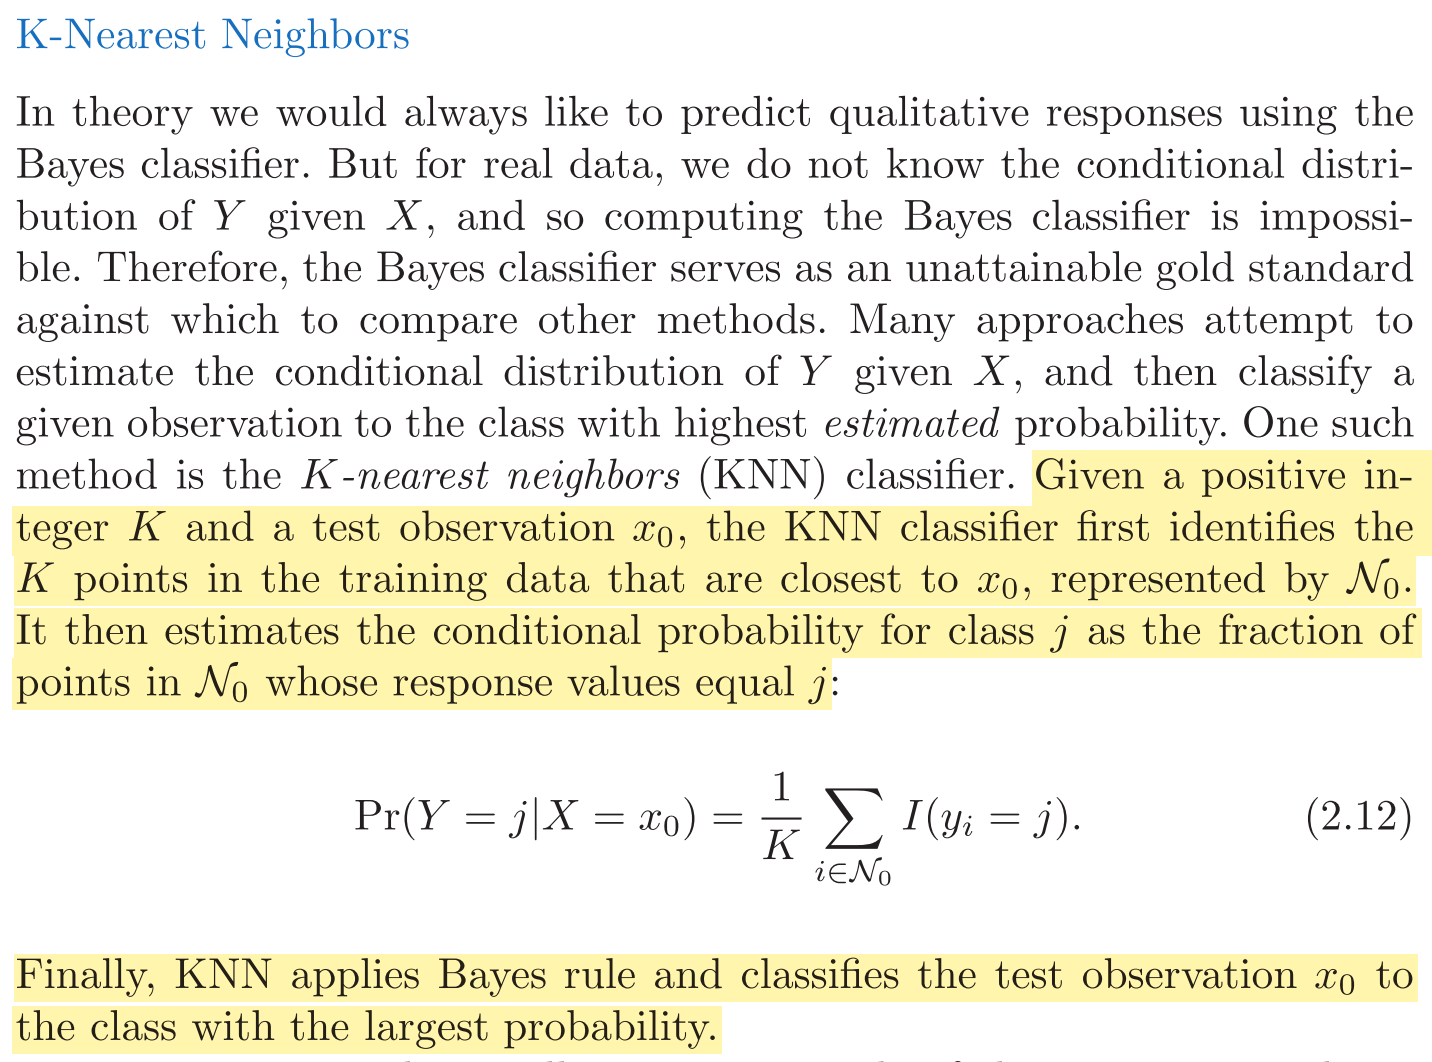
\includegraphics[width=.75\linewidth]{figures/KNN.png}
	\end{frame}

	\begin{frame}
	\frametitle{KNN How-To}
		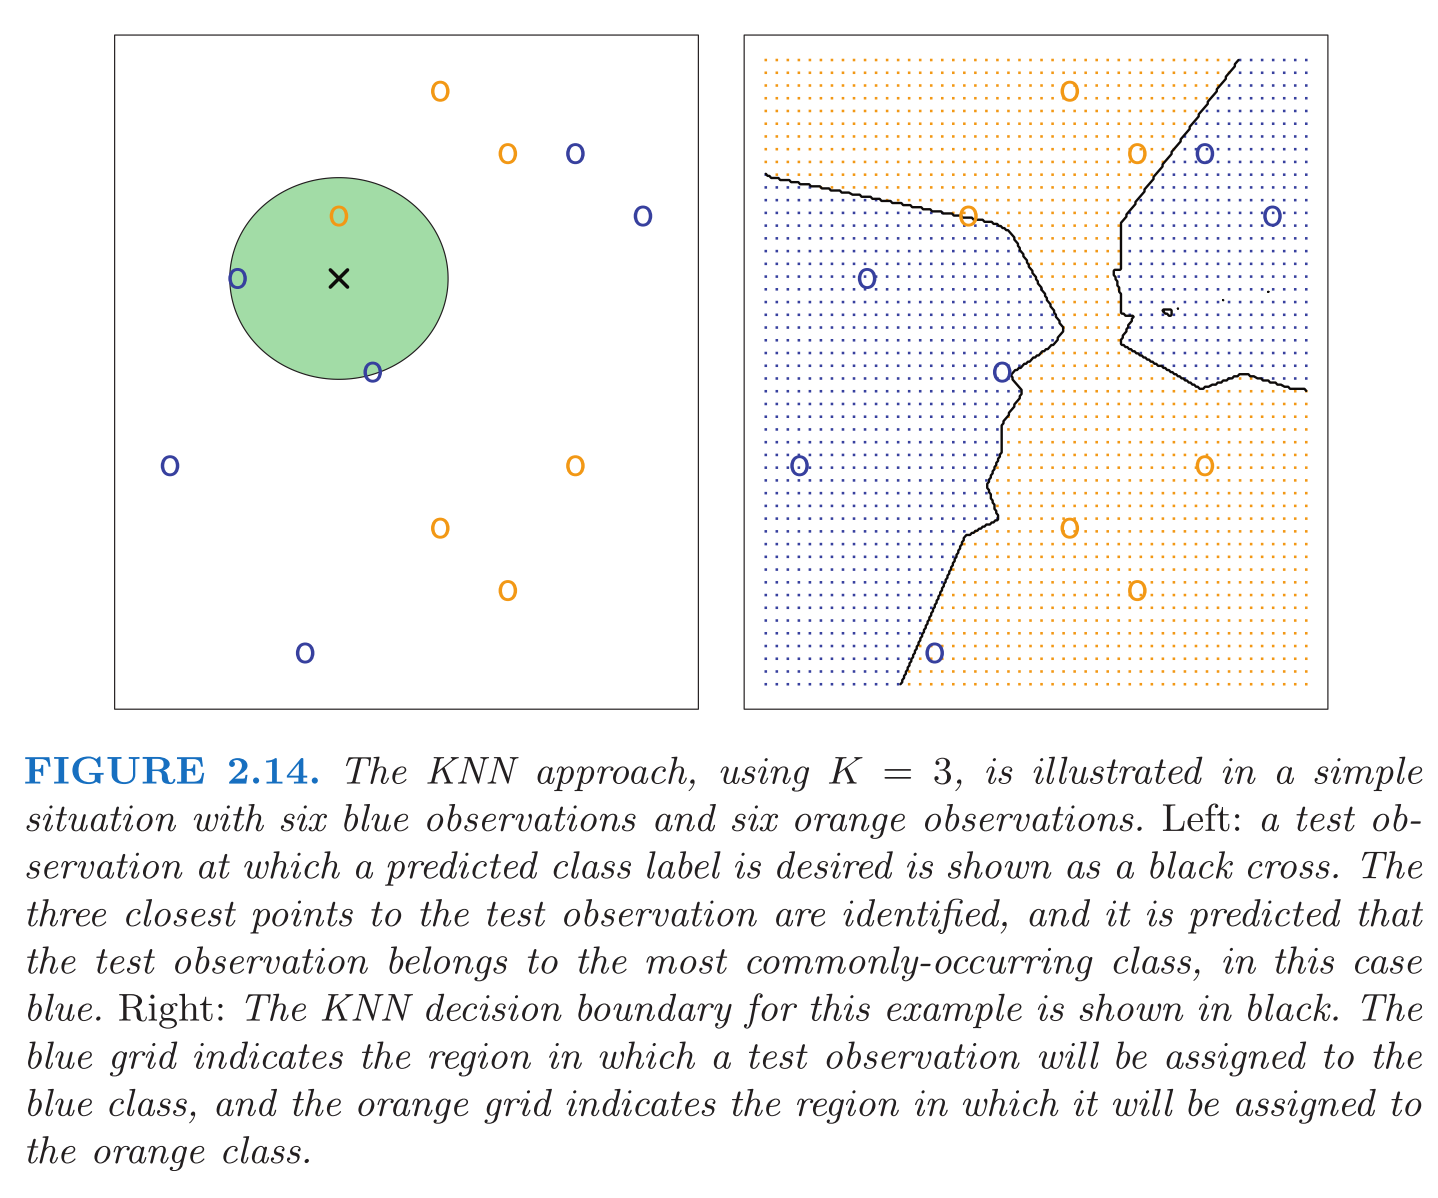
\includegraphics[width=.75\linewidth]{figures/KNN2.png}
		% For each of these, figure out if it's orange or blue.
	\end{frame}

	\begin{frame}
	\frametitle{KNN How-To}
		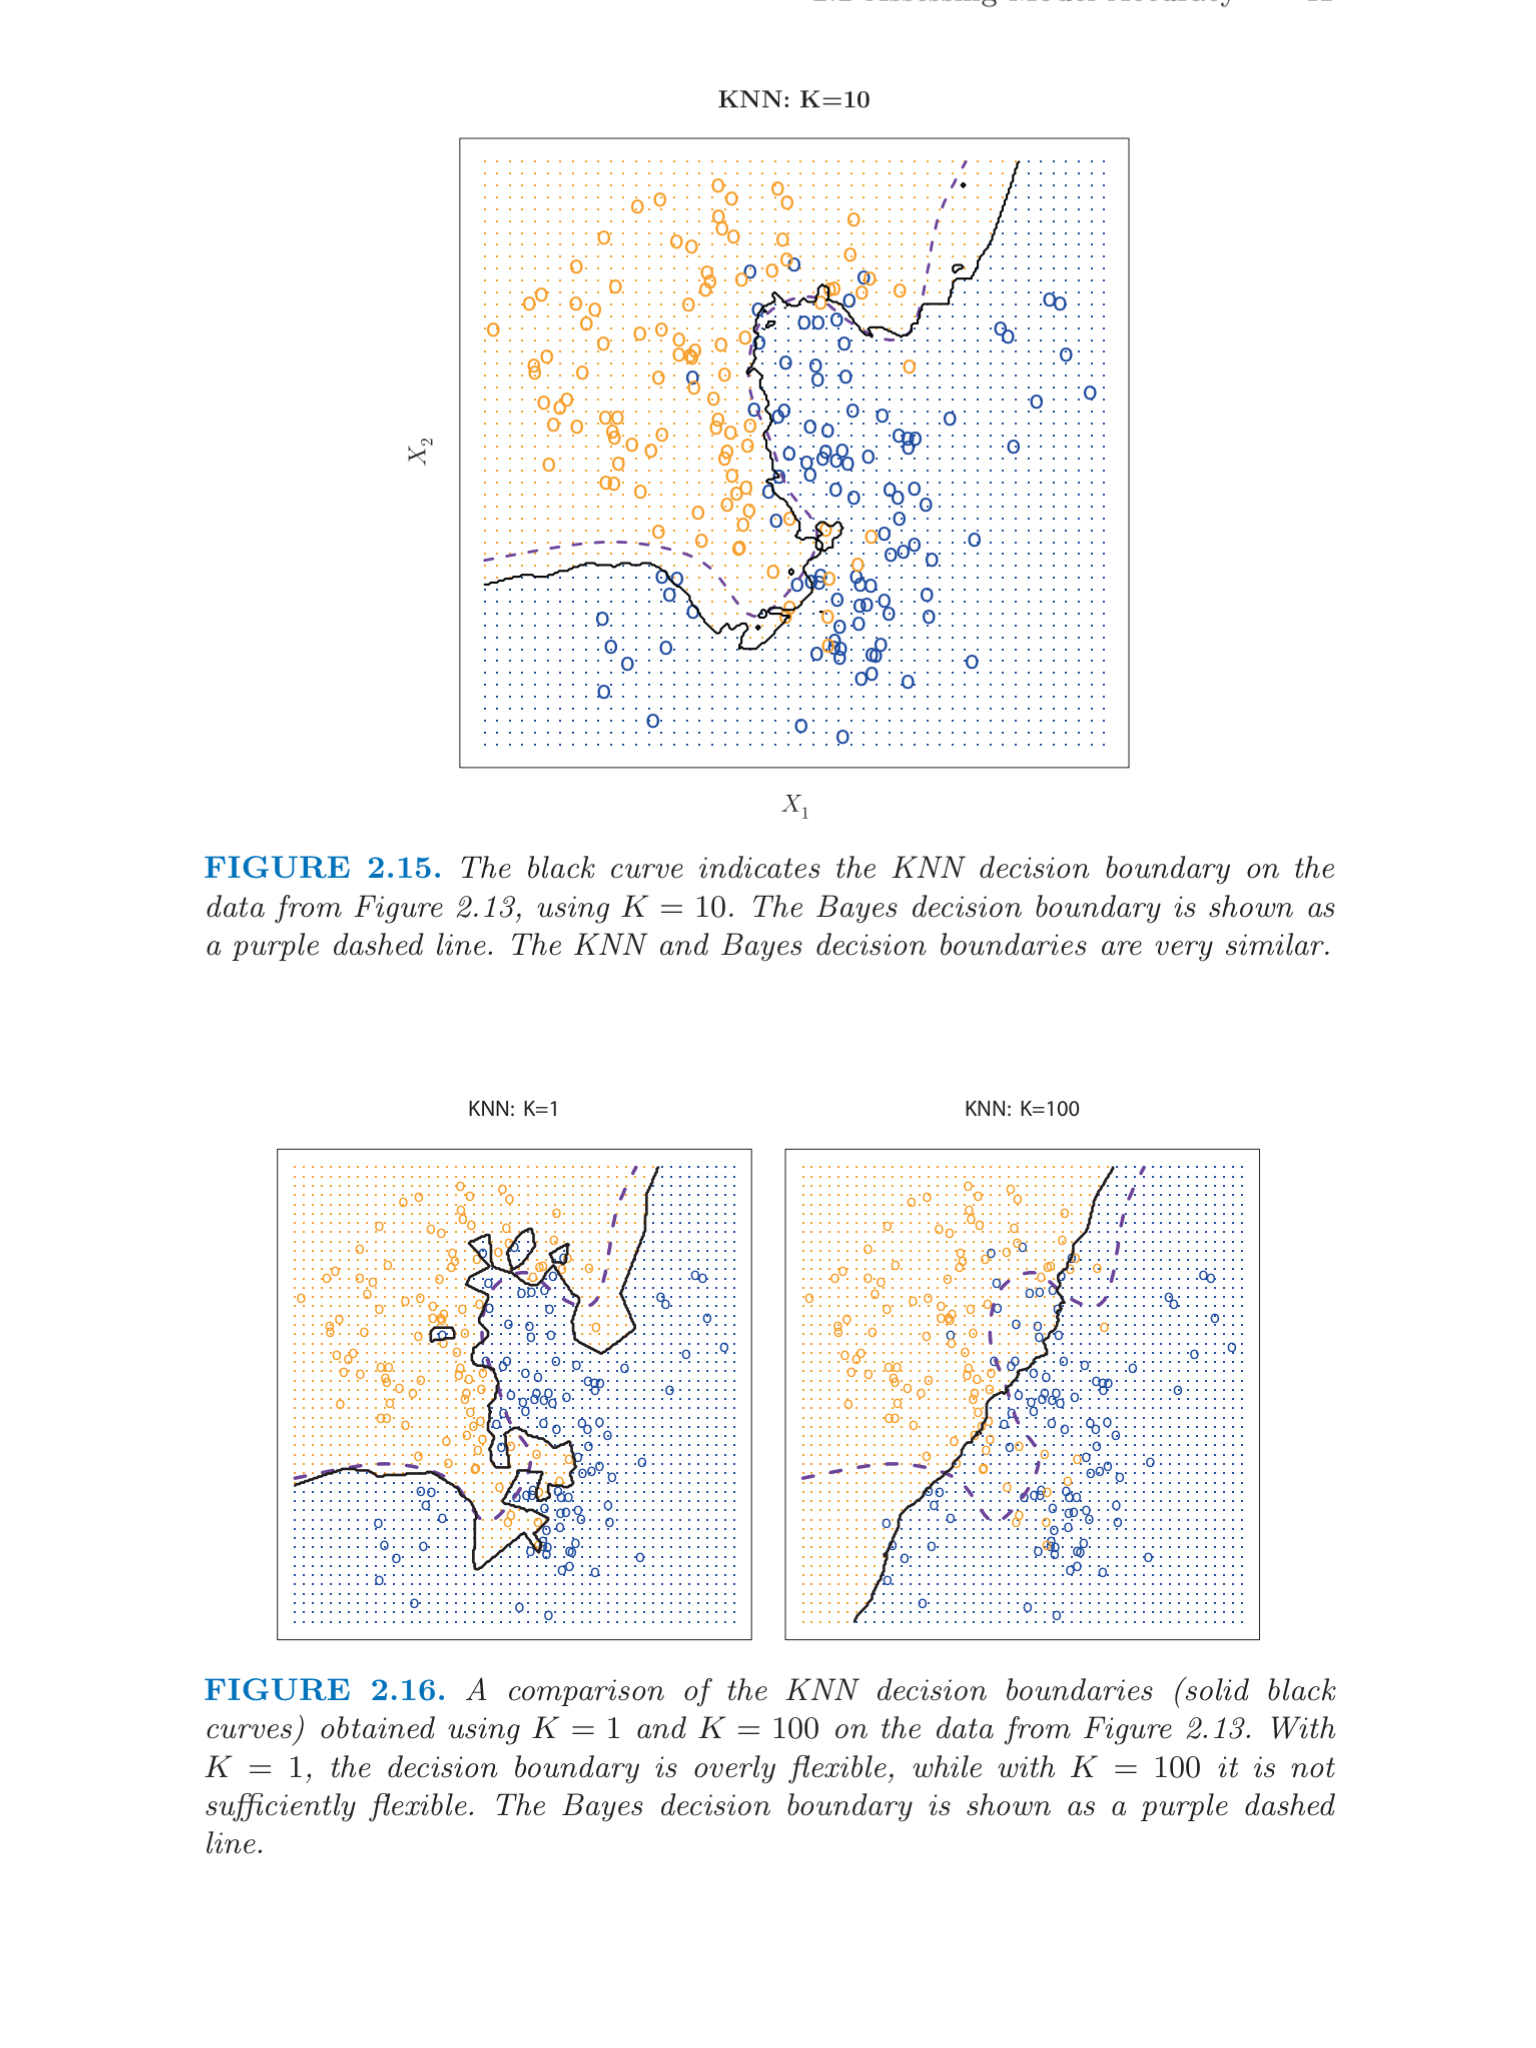
\includegraphics[width=.5\linewidth]{figures/KNN3.png}
	\end{frame}

	\begin{frame}
	\frametitle{KNN How-To}
		\begin{columns}
			\begin{column}{.5\linewidth}
				With our example data
			\end{column}
			\begin{column}{.5\linewidth}
				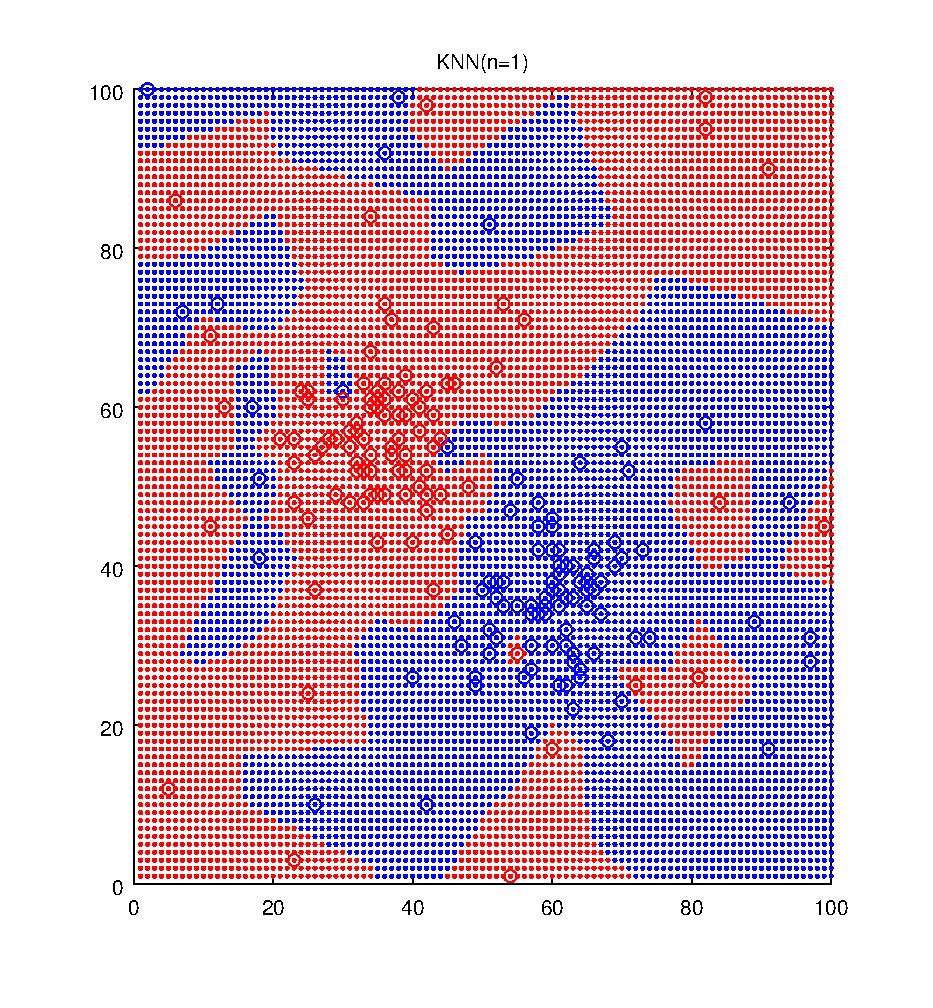
\includegraphics[width=1\linewidth]{figures/KNN1.eps}
			\end{column}
		\end{columns}
	\end{frame}
	\begin{frame}
	\frametitle{KNN How-To}
		\begin{columns}
			\begin{column}{.5\linewidth}
				With our example data
			\end{column}
			\begin{column}{.5\linewidth}
				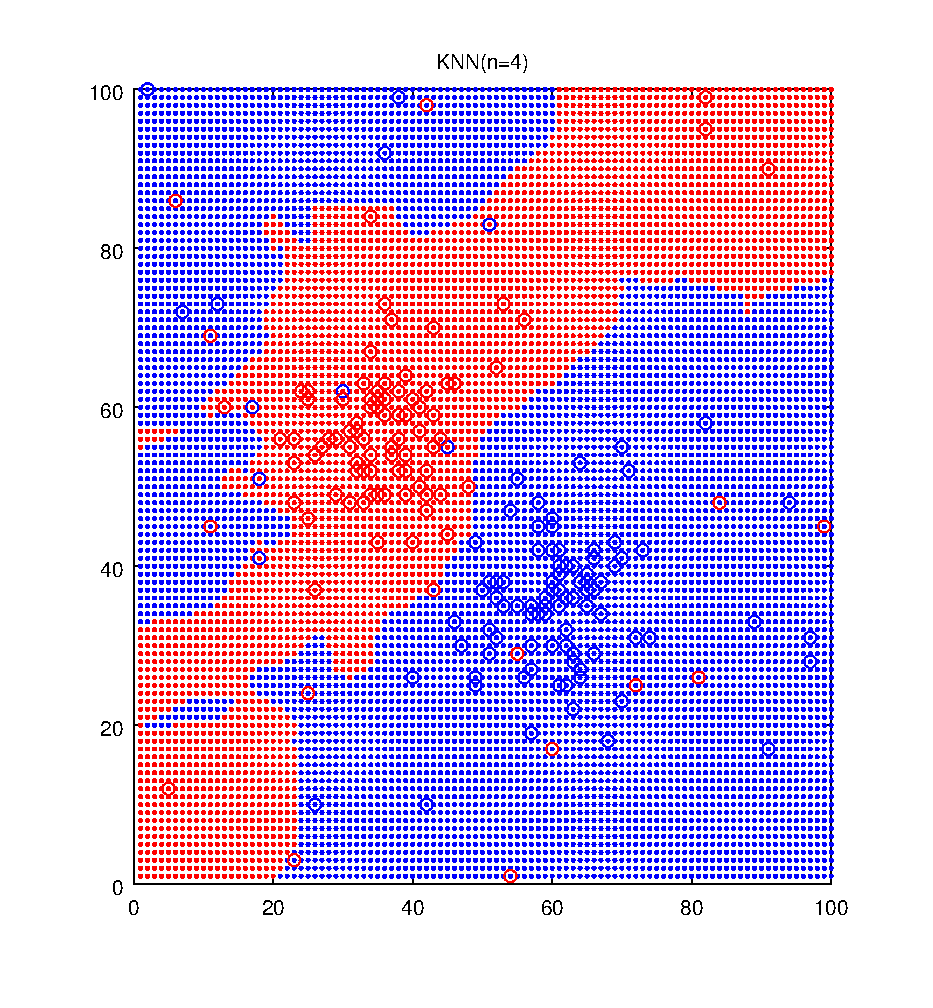
\includegraphics[width=1\linewidth]{figures/KNN4.eps}
			\end{column}
		\end{columns}
	\end{frame}

	\begin{frame}
	\frametitle{KNN How-To}
		\begin{columns}
			\begin{column}{.5\linewidth}
				With our example data

				See how this is averaging the boundaries out?
			\end{column}
			\begin{column}{.5\linewidth}
				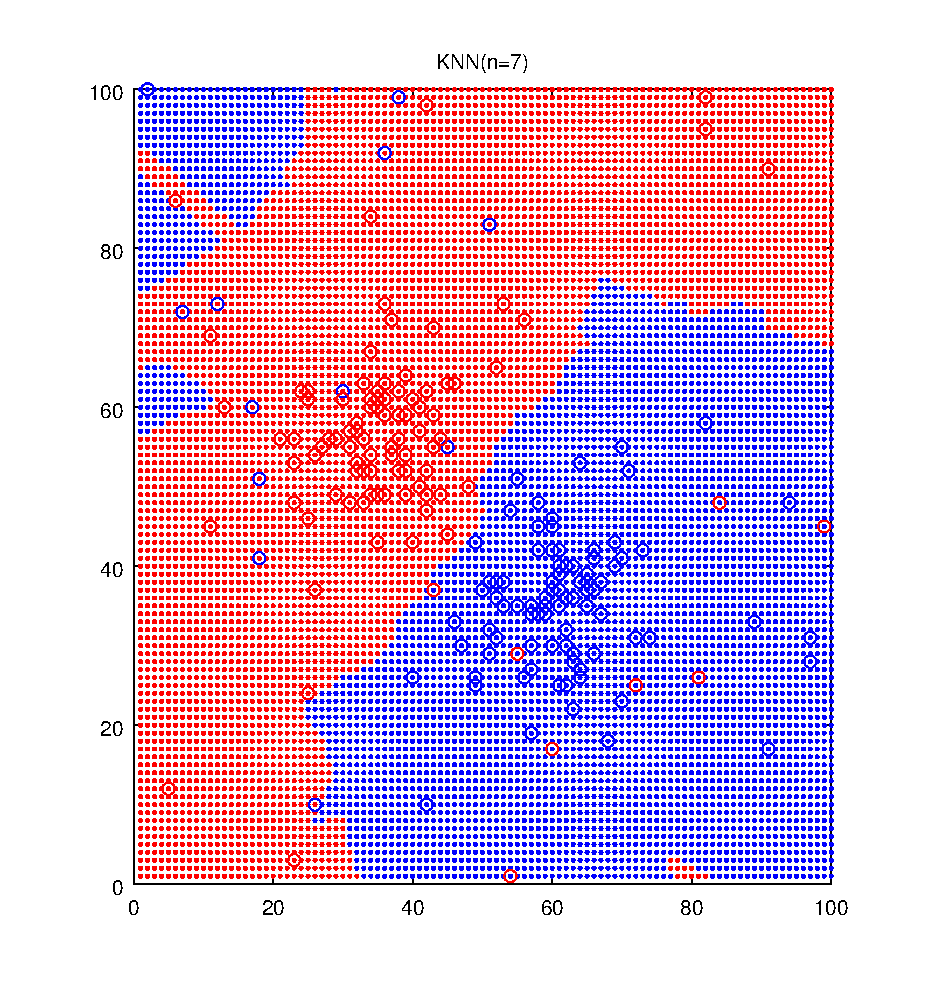
\includegraphics[width=1\linewidth]{figures/KNN7.eps}
			\end{column}
		\end{columns}
	\end{frame}

	\begin{frame}
	\frametitle{KNN How-To}
		\begin{columns}
			\begin{column}{.5\linewidth}
				With our example data

				Almost a single dividing line.  Almost.  But that's not really the goal.
			\end{column}
			\begin{column}{.5\linewidth}
				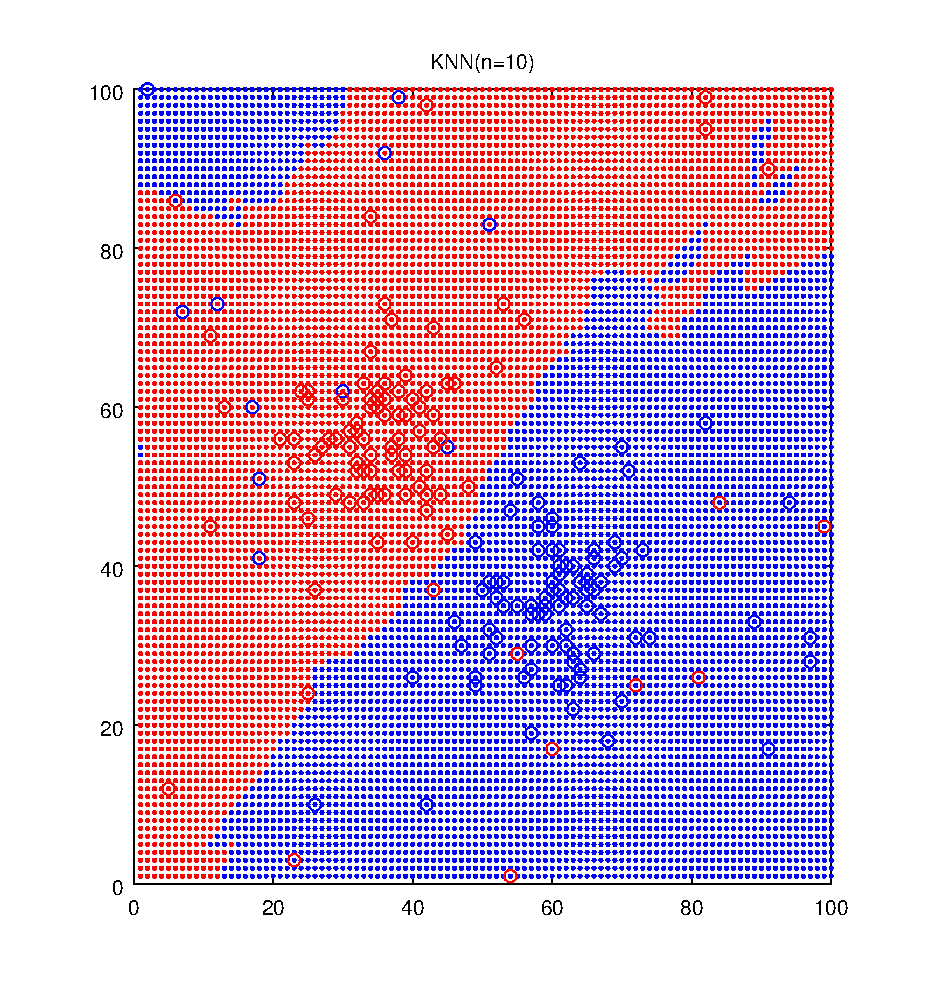
\includegraphics[width=1\linewidth]{figures/KNN10.eps}
			\end{column}
		\end{columns}
	\end{frame}

	\subsection{Comparing K-Means and KNN (Similarities, Differences?)}
	\begin{frame}
		\frametitle{Comparing K-Means and KNN}
		\begin{columns}
			\begin{column}{.5\linewidth}
				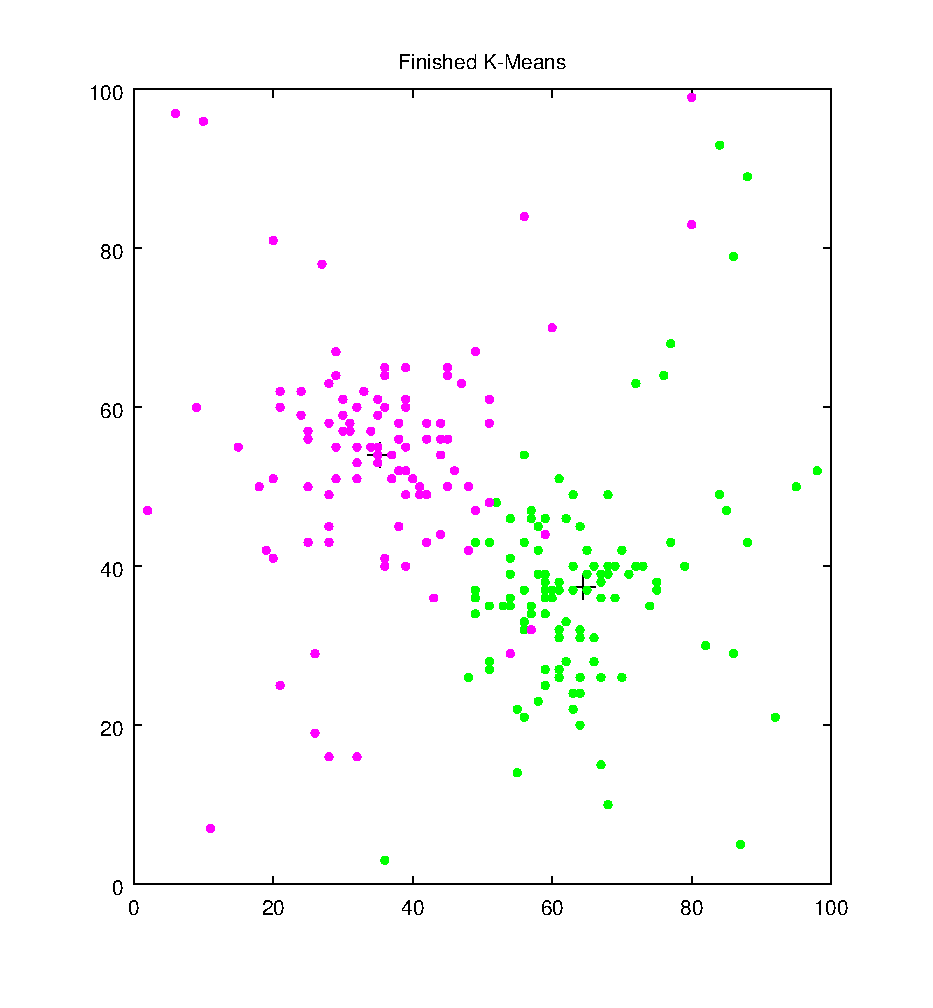
\includegraphics[width=1\linewidth]{figures/kmeans_done.eps}
			\end{column}
			\begin{column}{.5\linewidth}
				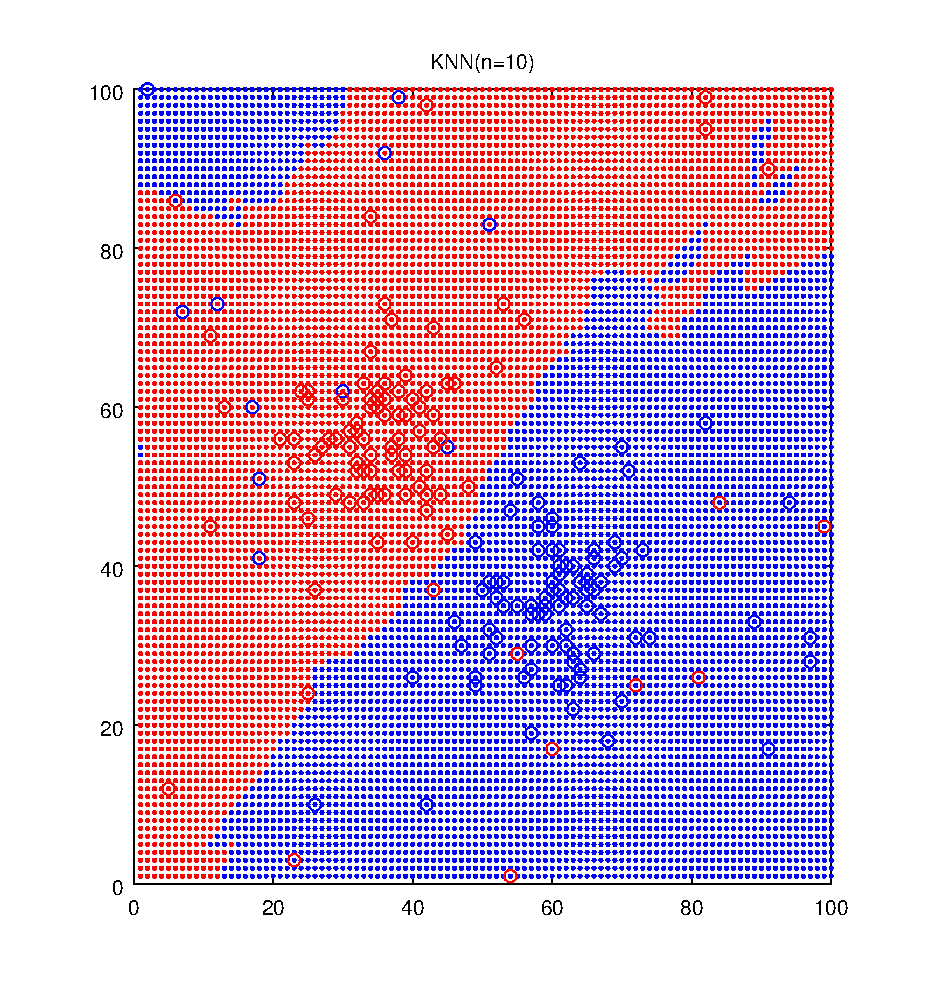
\includegraphics[width=1\linewidth]{figures/KNN10.eps}
			\end{column}
		\end{columns}
		If we introduced a new data point, then ... ?
	\end{frame}

	\begin{frame}
		\frametitle{Comparing K-Means and KNN}
		\begin{columns}
			\begin{column}{.5\linewidth}
				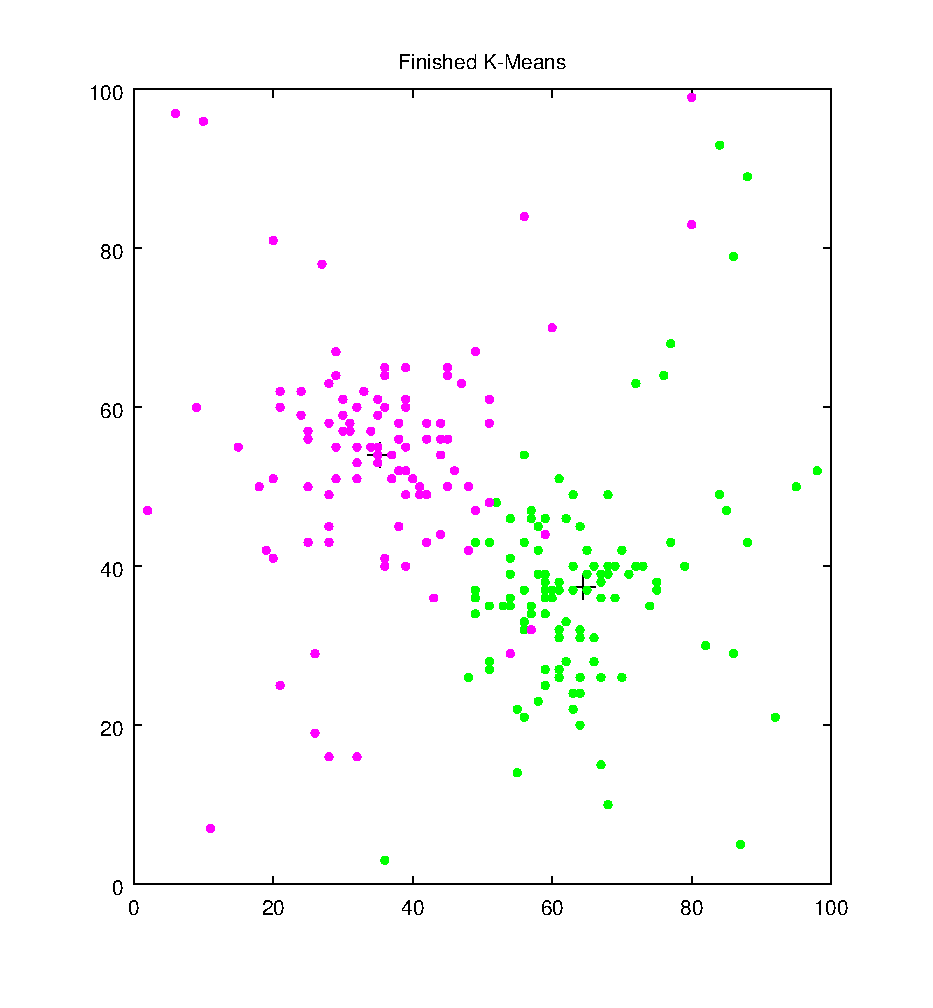
\includegraphics[width=1\linewidth]{figures/kmeans_done.eps}
				K-Means pulls data apart, after you have the data.
			\end{column}
			\begin{column}{.5\linewidth}
				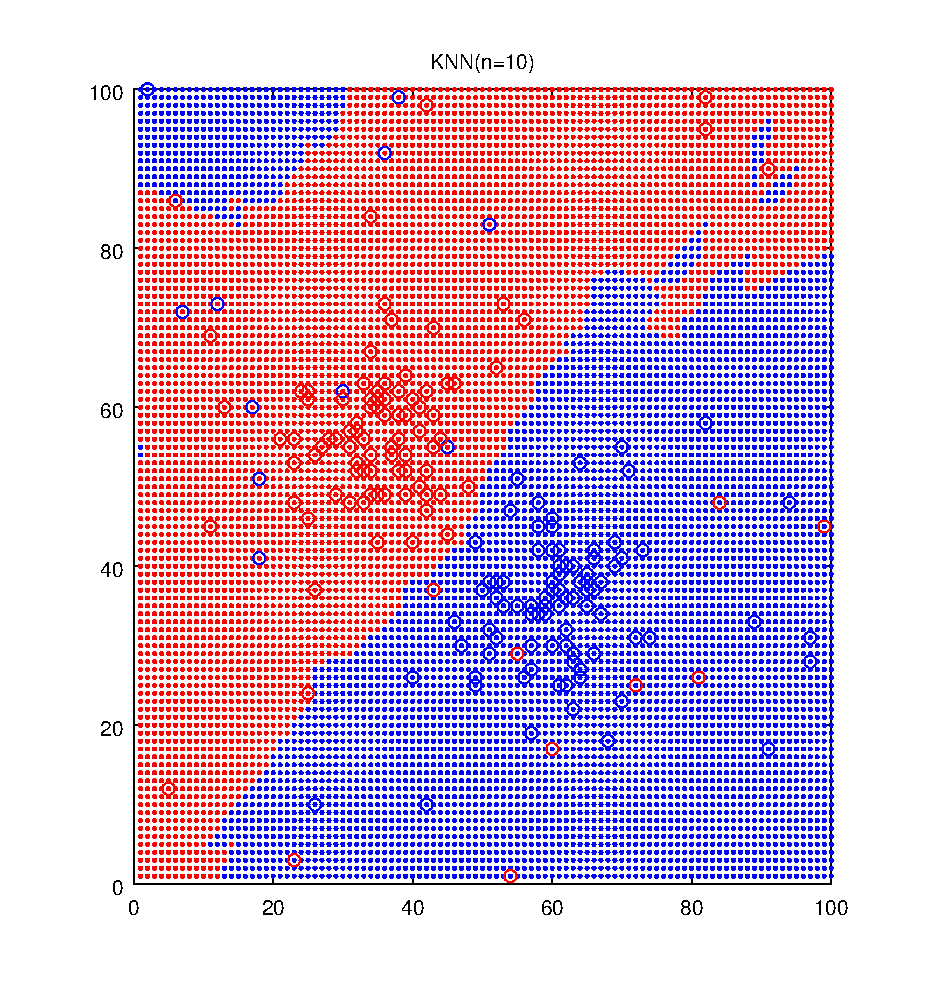
\includegraphics[width=1\linewidth]{figures/KNN10.eps}
				Use the labeled data, can be used as a live model.
			\end{column}
		\end{columns}
		
	\end{frame}

\end{document}
